\documentclass[aspectratio=169,10pt]{beamer}
\usetheme{mekatronik}
\renewcommand{\coursetitle}{Mechatronics and Robotics Engineering (50 h)}
\setweek{2}
\setday{2}{Robot Mechanisms II \& Robotic Manufacturing I}
\title[W2D2 -- IK, Jacobian, Dynamics, Motion, Automation]{Robot Mechanisms II and Introduction to Robotic Manufacturing}
\subtitle{4.4 Inverse kinematics \textbullet\ 4.5 Jacobian \& statics \textbullet\ 4.6 Dynamics \textbullet\ 4.7 Motion \& trajectories \textbullet\ 5.1 Flexible automation}
\author{Mechatronics and Robotics Engineering Programme}
\institute{Week 2 \textperiodcentered{} Day 2}
\date{2 weeks \textperiodcentered{} 10 days \textperiodcentered{} 50 hours}

% ---- local helpers -------------------------------------------------
\tikzset{
  blk/.style={draw=mkBlue,fill=mkPale,rounded corners=1.5pt,minimum height=7mm,minimum width=12mm,font=\scriptsize,align=center,line width=.6pt},
  blko/.style={blk,draw=mkOrange,fill=mkCream},
  sig/.style={-{Latex[length=2mm]},mkNavy,line width=.6pt},
  vec/.style={-{Latex[length=2.2mm]},line width=1pt},
  lnk/.style={line width=3pt,mkBlue,line cap=round},
  lnko/.style={line width=3pt,mkOrange,line cap=round},
  jnt/.style={circle,draw=mkNavy,fill=white,line width=.8pt,inner sep=1.6pt},
  lab/.style={font=\scriptsize,text=mkNavy},
}
% 2-link arm: \arm{theta1}{theta2}{style}  (L1=2.4, L2=1.8 drawing units = 0.4 m, 0.3 m)
\newcommand{\arm}[3]{%
  \draw[#3] (0,0) -- ++(#1:2.4) coordinate (E) -- ++(#1+#2:1.8) coordinate (T);
  \node[jnt] at (0,0) {}; \node[jnt] at (E) {}; \fill[mkOrange] (T) circle (1.6pt);}
\newcommand{\base}{\fill[pattern=north east lines,pattern color=mkGray] (-.35,-.25) rectangle (.35,-.08);
  \draw[mkGray,line width=.8pt] (-.35,-.08) -- (.35,-.08);}
\newcommand{\src}[1]{\par\vfill\hfill{\color{mkGray}\fontsize{6}{7}\selectfont #1}}
\newcommand{\gofurther}[1]{\par\vspace{1mm}{\scriptsize\color{mkGray}\textbf{\color{mkMid}Going further:} #1\par}}
\pgfplotsset{every axis/.append style={label style={font=\scriptsize}}}
% photo credits (short on slide, long on credits frame)
\newcommand{\creditagv}{AGV pallet stacker. Marc Auledas Noguera, CC BY 4.0, via Wikimedia Commons}
\newcommand{\creditagvlong}{``Jungheinrich ERC 213a 217a Automated Guided Vehicle.jpg'', Marc Auledas Noguera (Auledas), CC BY 4.0}
\newcommand{\creditwelding}{Spot welding of car bodies, BMW plant Leipzig. BMW Werk Leipzig, CC BY-SA 2.0 de, via Wikimedia Commons}
\newcommand{\creditweldinglong}{``BMW Leipzig MEDIA 050719 Download Karosseriebau max.jpg'', BMW Werk Leipzig, CC BY-SA 2.0 de}

\begin{document}

\begin{frame}[plain]\titlepage\end{frame}

% =====================================================================
\begin{frame}[t]{Agenda and learning outcomes}
\begin{columns}[T,onlytextwidth]
\column{.52\textwidth}
\footnotesize
\begin{tabularx}{\linewidth}{@{}l X r@{}}
\toprule
\textbf{Code} & \textbf{Session} & \textbf{Time}\\
\midrule
4.4 & Inverse kinematics: 2-link solution, multiple solutions, reach & 1 h\\
4.5 & Velocity kinematics: Jacobian, singularities, statics & 1 h\\
4.6 & Introduction to robot dynamics & 1 h\\
4.7 & Motion systems and trajectory planning & 1 h\\
5.1 & Robotic manufacturing and flexible automation & 1 h\\
\midrule
 & \textbf{Total} (+ 10-min breaks about every hour) & \textbf{5 h}\\
\bottomrule
\end{tabularx}\\[2mm]
\begin{notebox}
\textbf{One robot all day:} a planar 2-link arm with $L_1=\SI{0.4}{m}$, $L_2=\SI{0.3}{m}$
(think of a SCARA seen from above, or a shoulder + elbow seen from the side).
\end{notebox}
\column{.45\textwidth}
\begin{keybox}[By the end of today you can \ldots]
\small
\checkitem\ solve the 2-link inverse kinematics and find both solutions\\
\checkitem\ decide whether a point is reachable\\
\checkitem\ build the Jacobian and spot singularities\\
\checkitem\ calculate joint torques from a tip force ($\tau=J^\mathsf{T}F$)\\
\checkitem\ estimate gravity torques and explain payload effects\\
\checkitem\ compare PTP, linear and circular moves; compute an AMR's motion\\
\checkitem\ distinguish fixed, programmable and flexible automation
\end{keybox}
\end{columns}
\end{frame}

% =====================================================================
\begin{frame}[t]{What we learned so far (W2D1)}
\begin{columns}[T,onlytextwidth]
\column{.52\textwidth}
\begin{itemize}\small
\item \textbf{3.7} Joints are springy: resonance, notch filters
\item \textbf{4.1} Robot anatomy: joints, DOF, workspace; articulated, SCARA, gantry, delta, cobots, AMRs
\item \textbf{4.2} Pose = position + orientation; rotation matrix $R$, homogeneous transform $T$
\item \textbf{4.3} Forward kinematics: chain the transforms, joint angles $\rightarrow$ tool pose
\end{itemize}
\begin{notebox}
Today we turn the question around (where must the joints go?), then add speed, force and
mass, and finally zoom out to the whole factory.
\end{notebox}
\column{.45\textwidth}
\centering
\begin{tikzpicture}[scale=.9]
\draw[->,mkGray] (0,0) -- (3.2,0) node[right,lab] {$x_0$};
\draw[->,mkGray] (0,0) -- (0,2.4) node[above,lab] {$y_0$};
\begin{scope}[shift={(2,1.2)},rotate=35]
\draw[vec,mkOrange] (0,0) -- (1,0) node[right,lab] {$x_1$};
\draw[vec,mkOrange] (0,0) -- (0,1) node[above,lab] {$y_1$};
\end{scope}
\draw[vec,mkBlue] (0,0) -- (2,1.2) node[midway,above left,lab] {$\bm p$};
\draw[mkMid] (2.6,1.2) arc (0:35:.6) node[midway,right,lab] {$\theta$};
\draw[mkGray,dashed] (2,1.2) -- (2.8,1.2);
\node[lab,align=center] at (1.6,-.7) {$T=\begin{bmatrix} R & \bm p\\ \bm 0^\mathsf{T} & 1\end{bmatrix}$};
\end{tikzpicture}
\end{columns}
\end{frame}

\begin{frame}[t]{Recap: forward kinematics of our 2-link arm}
\begin{columns}[T,onlytextwidth]
\column{.5\textwidth}
\begin{itemize}\small
\item Joint angles $\theta_1$ (shoulder), $\theta_2$ (elbow, relative to link 1)
\item Tip position = sum of two link vectors
\end{itemize}
\begin{eqbox}
\[
\begin{aligned}
x &= L_1\cos\theta_1 + L_2\cos(\theta_1+\theta_2)\\
y &= L_1\sin\theta_1 + L_2\sin(\theta_1+\theta_2)
\end{aligned}
\]
\end{eqbox}
\begin{itemize}\small
\item Example: $\theta_1=0$, $\theta_2=\SI{90}{\degree}$ $\Rightarrow$ $x=\SI{0.4}{m}$, $y=\SI{0.3}{m}$
\item Short-hand: $c_1=\cos\theta_1$, $s_{12}=\sin(\theta_1+\theta_2)$
\end{itemize}
\column{.46\textwidth}
\centering
\begin{tikzpicture}[scale=.85]
\draw[->,mkGray] (-.3,0) -- (4.6,0) node[right,lab] {$x$};
\draw[->,mkGray] (0,-.3) -- (0,3.6) node[above,lab] {$y$};
\arm{25}{60}{lnk}
\node[lab,above left] at ($(0,0)!.5!(E)$) {$L_1$};
\node[lab,right] at ($(E)!.5!(T)$) {$L_2$};
\draw[mkMid] (.8,0) arc (0:25:.8) node[midway,right,lab] {$\theta_1$};
\draw[mkGray,dashed] (E) -- ++(25:1);
\draw[mkOrange] ($(E)+(25:.6)$) arc (25:85:.6) node[midway,above right,lab] {$\theta_2$};
\node[lab,right] at (T) {$(x,y)$};
\base
\end{tikzpicture}
\end{columns}
\end{frame}

% =====================================================================
\section{4.4 Inverse kinematics}

\begin{frame}[t]{The inverse question: where must the joints go?}
\begin{columns}[T,onlytextwidth]
\column{.5\textwidth}
\begin{itemize}\small
\item \term{Forward kinematics (FK)}: joints $\rightarrow$ tool pose. One answer, always.
\item \term{Inverse kinematics (IK)}: desired tool pose $\rightarrow$ joint angles.
\item IK is what we actually need: tasks are given in the world (``pick the part at $x,y$'')
\item Analogy: reaching for a cup -- you think of the cup, your brain finds shoulder and elbow angles
\end{itemize}
\begin{keybox}[Why IK is harder]
Nonlinear (sin, cos), may have \hl{0, 1, 2 or more} answers.
\end{keybox}
\column{.46\textwidth}
\centering
\begin{tikzpicture}
\node[blk,minimum width=22mm,minimum height=10mm] (J) at (0,0) {Joint space\\$(\theta_1,\theta_2)$};
\node[blko,minimum width=22mm,minimum height=10mm] (C) at (0,-3) {Task space\\$(x,y)$};
\draw[sig] ([xshift=-6mm]J.south) to[bend right=25] node[left,lab,align=right] {FK\\easy, unique} ([xshift=-6mm]C.north);
\draw[sig,mkOrange] ([xshift=6mm]C.north) to[bend right=25] node[right,lab,align=left] {IK\\hard, several\\answers} ([xshift=6mm]J.south);
\end{tikzpicture}
\end{columns}
\end{frame}

\begin{frame}[t]{Reachability: the workspace of the 2-link arm}
\begin{columns}[T,onlytextwidth]
\column{.5\textwidth}
\begin{itemize}\small
\item Distance from base to target: $r=\sqrt{x^2+y^2}$
\item Fully stretched: $r_{\max}=L_1+L_2=\SI{0.7}{m}$
\item Fully folded: $r_{\min}=|L_1-L_2|=\SI{0.1}{m}$
\end{itemize}
\begin{eqbox}
\[ |L_1-L_2| \;\le\; \sqrt{x^2+y^2} \;\le\; L_1+L_2 \]
\end{eqbox}
\begin{itemize}\small
\item Outside the ring: \hl{no solution} (unreachable)
\item Real joint limits cut the ring further
\end{itemize}
\column{.46\textwidth}
\centering
\begin{tikzpicture}[scale=.62]
\fill[mkPale,even odd rule] (0,0) circle (4.2) (0,0) circle (.6);
\draw[mkMid] (0,0) circle (4.2); \draw[mkMid] (0,0) circle (.6);
\draw[->,mkGray] (-4.6,0) -- (4.7,0) node[right,lab] {$x$};
\draw[->,mkGray] (0,-4.6) -- (0,4.7) node[above,lab] {$y$};
\draw[mkOrange,<->] (0,0) -- (-35:4.2) node[pos=.6,below left,lab] {$\SI{0.7}{m}$};
\draw[lnk] (0,0) -- (40:2.4) -- ++(40:1.8);
\node[jnt] at (0,0) {};
\fill[mkGreen] (-2.2,2.4) circle (2.5pt) node[above,lab] {reachable};
\fill[mkRed] (3.6,3.4) circle (2.5pt) node[right,lab] {not reachable};
\node[lab,fill=white,inner sep=1pt] at (1.2,-.75) {hole $\SI{0.1}{m}$};
\end{tikzpicture}
\end{columns}
\end{frame}

\begin{frame}[t]{Refresher: law of cosines and the two-argument arctangent}
\begin{columns}[T,onlytextwidth]
\column{.5\textwidth}
\begin{defbox}[Refresher: law of cosines]
For a triangle with sides $a,b,c$ and angle $\gamma$ opposite $c$:
\[ c^2 = a^2 + b^2 - 2ab\cos\gamma \]
Pythagoras is the special case $\gamma=\SI{90}{\degree}$.
\end{defbox}
\begin{defbox}[Refresher: atan2]
$\operatorname{atan2}(y,x)$ = angle of the point $(x,y)$, in $(-\SI{180}{\degree},\SI{180}{\degree}]$.
Unlike $\arctan(y/x)$ it knows the \hl{quadrant}.
\end{defbox}
\column{.46\textwidth}
\centering
\begin{tikzpicture}[scale=.8]
\draw[->,mkGray] (-2.6,0) -- (2.8,0) node[right,lab] {$x$};
\draw[->,mkGray] (0,-1.6) -- (0,2.2) node[above,lab] {$y$};
\draw[vec,mkBlue] (0,0) -- (1.6,1.2) node[right,lab] {$(1,1)$: $\SI{45}{\degree}$};
\draw[vec,mkOrange] (0,0) -- (-1.6,-1.2) node[below,lab] {$(-1,-1)$: $-\SI{135}{\degree}$};
\node[lab,align=center,text width=5.2cm] at (0,-2.4) {$\arctan(\tfrac{1}{1})=\arctan(\tfrac{-1}{-1})=\SI{45}{\degree}$: the plain arctangent cannot tell these two apart.};
\end{tikzpicture}
\end{columns}
\end{frame}

\begin{frame}[t]{Geometric solution, step 1: the elbow angle}
\begin{columns}[T,onlytextwidth]
\column{.52\textwidth}
\begin{itemize}\small
\item Base, elbow and tip form a triangle with sides $L_1$, $L_2$, $r$
\item Apply the law of cosines to this triangle (interior angle at the elbow $=\SI{180}{\degree}-\theta_2$):
\end{itemize}
\begin{eqbox}
\[ \cos\theta_2 = \frac{x^2+y^2-L_1^2-L_2^2}{2L_1L_2} \]
\end{eqbox}
\begin{itemize}\small
\item If the right side is outside $[-1,1]$: target \hl{unreachable}
\item $\theta_2=\pm\arccos(\ldots)$ $\rightarrow$ \hl{two} elbow solutions
\end{itemize}
\column{.44\textwidth}
\centering
\begin{tikzpicture}[scale=.85]
\draw[->,mkGray] (-.3,0) -- (4.4,0) node[right,lab] {$x$};
\draw[->,mkGray] (0,-.3) -- (0,3.4) node[above,lab] {$y$};
\arm{20}{75}{lnk}
\draw[mkOrange,dashed,line width=.8pt] (0,0) -- (T) node[pos=.55,above left,lab] {$r$};
\node[lab,below right] at ($(0,0)!.5!(E)$) {$L_1$};
\node[lab,right] at ($(E)!.5!(T)$) {$L_2$};
\draw[mkGray,dashed] (E) -- ++(20:.9);
\draw[mkOrange] ($(E)+(20:.5)$) arc (20:95:.5) node[pos=.6,above right,lab] {$\theta_2$};
\node[lab,right] at (T) {$(x,y)$};
\base
\end{tikzpicture}
\end{columns}
\end{frame}

\begin{frame}[t]{Geometric solution, step 2: the shoulder angle}
\begin{columns}[T,onlytextwidth]
\column{.52\textwidth}
\begin{itemize}\small
\item $\theta_1$ = (direction to target) $-$ (angle between link 1 and the line to the target)
\end{itemize}
\begin{eqbox}
\[ \begin{aligned} \theta_1 &= \beta-\psi\\ \beta &= \operatorname{atan2}(y,\,x)\\ \psi &= \operatorname{atan2}\!\big(L_2\sin\theta_2,\;L_1+L_2\cos\theta_2\big)\end{aligned} \]
\end{eqbox}
\begin{itemize}\small
\item Use the $\theta_2$ from step 1 (each sign gives its own $\theta_1$)
\item Always use \texttt{atan2}, never $\arctan$ of a ratio
\item Always check: put the answer back into FK
\end{itemize}
\column{.44\textwidth}
\centering
\begin{tikzpicture}[scale=.85]
\draw[->,mkGray] (-.3,0) -- (4.4,0) node[right,lab] {$x$};
\draw[->,mkGray] (0,-.3) -- (0,3.4) node[above,lab] {$y$};
\arm{20}{75}{lnk}
\draw[mkOrange,dashed,line width=.8pt] (0,0) -- (T);
\draw[mkMid] (1.3,0) arc (0:20:1.3) node[pos=.5,right,lab] {$\theta_1$};
\draw[mkOrange] (0:2.0) arc (0:51.3:2.0);
\node[lab,text=mkOrange] at (2.3,1.6) {$\beta$};
\draw[mkGreen,line width=.8pt] (20:.8) arc (20:51.3:.8) node[pos=.5,above right,lab,text=mkGreen] {$\psi$};
\base
\end{tikzpicture}
\end{columns}
\end{frame}

\begin{frame}[t]{Two solutions: elbow up and elbow down}
\begin{columns}[T,onlytextwidth]
\column{.48\textwidth}
\begin{itemize}\small
\item Same tip position, two arm shapes (mirror images about the line base--target)
\item $\theta_2>0$: one shape, $\theta_2<0$: the other
\item On a SCARA these are called \term{right-handed} and \term{left-handed}
\item The robot program must say which one -- the \term{configuration}
\item On the workspace boundary ($r=r_{\max}$) the two merge into one
\end{itemize}
\column{.48\textwidth}
\centering
\begin{tikzpicture}[scale=.95]
\draw[->,mkGray] (-.3,0) -- (4.2,0) node[right,lab] {$x$};
\draw[->,mkGray] (0,-.3) -- (0,3.6) node[above,lab] {$y$};
\arm{2.48}{67.98}{lnk}
\node[lab,below,text=mkBlue] at (E) {elbow down};
\arm{59.45}{-67.98}{lnko}
\node[lab,above left,text=mkOrange] at (E) {elbow up};
\draw[mkGray,dashed] (0,0) -- (T);
\node[lab,right] at (T) {$(0.5,\,0.3)\,$m};
\base
\end{tikzpicture}
\end{columns}
\end{frame}

\begin{frame}[t]{Worked example: IK for the target $(0.5,\,0.3)$ m}
\begin{columns}[T,onlytextwidth]
\column{.56\textwidth}
\small
\begin{enumerate}
\item Reach: $r=\sqrt{0.25+0.09}=\SI{0.583}{m}$, inside $[0.1,\,0.7]$ \checkmark
\item $\cos\theta_2=\dfrac{0.34-0.16-0.09}{2\cdot0.4\cdot0.3}=\dfrac{0.09}{0.24}=0.375$\\
 $\Rightarrow\theta_2=\pm\SI{68.0}{\degree}$
\item $\beta=\operatorname{atan2}(0.3,0.5)=\SI{31.0}{\degree}$;\\
 $\psi=\operatorname{atan2}(0.3\cdot0.927,\;0.4+0.3\cdot0.375)=\operatorname{atan2}(0.278,0.513)=\SI{28.5}{\degree}$
\item Elbow down: $\theta_1=31.0-28.5=\SI{2.5}{\degree}$, $\theta_2=+\SI{68.0}{\degree}$\\
 Elbow up: $\theta_1=31.0+28.5=\SI{59.5}{\degree}$, $\theta_2=-\SI{68.0}{\degree}$
\end{enumerate}
\column{.4\textwidth}
\begin{keybox}[Check with FK (elbow down)]
$x=0.4\cos 2.5^\circ+0.3\cos 70.5^\circ$\\
$\phantom{x}=0.400+0.100=\SI{0.50}{m}$ \checkmark\\[1mm]
$y=0.4\sin 2.5^\circ+0.3\sin 70.5^\circ$\\
$\phantom{y}=0.017+0.283=\SI{0.30}{m}$ \checkmark
\end{keybox}
\begin{notebox}
For the elbow-up case $\psi$ changes sign, because $\sin\theta_2<0$.
\end{notebox}
\end{columns}
\end{frame}

\begin{frame}[t]{IK of real robots}
\begin{columns}[T,onlytextwidth]
\column{.56\textwidth}
\begin{itemize}\small
\item 6-axis arm: position \emph{and} orientation $\rightarrow$ up to \hl{8} solutions (shoulder front/back, elbow up/down, wrist flip/no flip)
\item Most industrial arms have a \term{spherical wrist} (last 3 axes meet in a point) $\rightarrow$ IK splits into ``arm finds the position, wrist finds the orientation''
\item Joint limits remove some solutions
\item Controller picks the one matching the programmed configuration, or the closest to the current pose
\end{itemize}
\gofurther{Robots without a closed-form solution use \emph{numerical IK}: guess, compute the FK error, correct with the Jacobian (next session), repeat. Redundant robots (7 axes) have infinitely many solutions.}
\column{.4\textwidth}
\centering
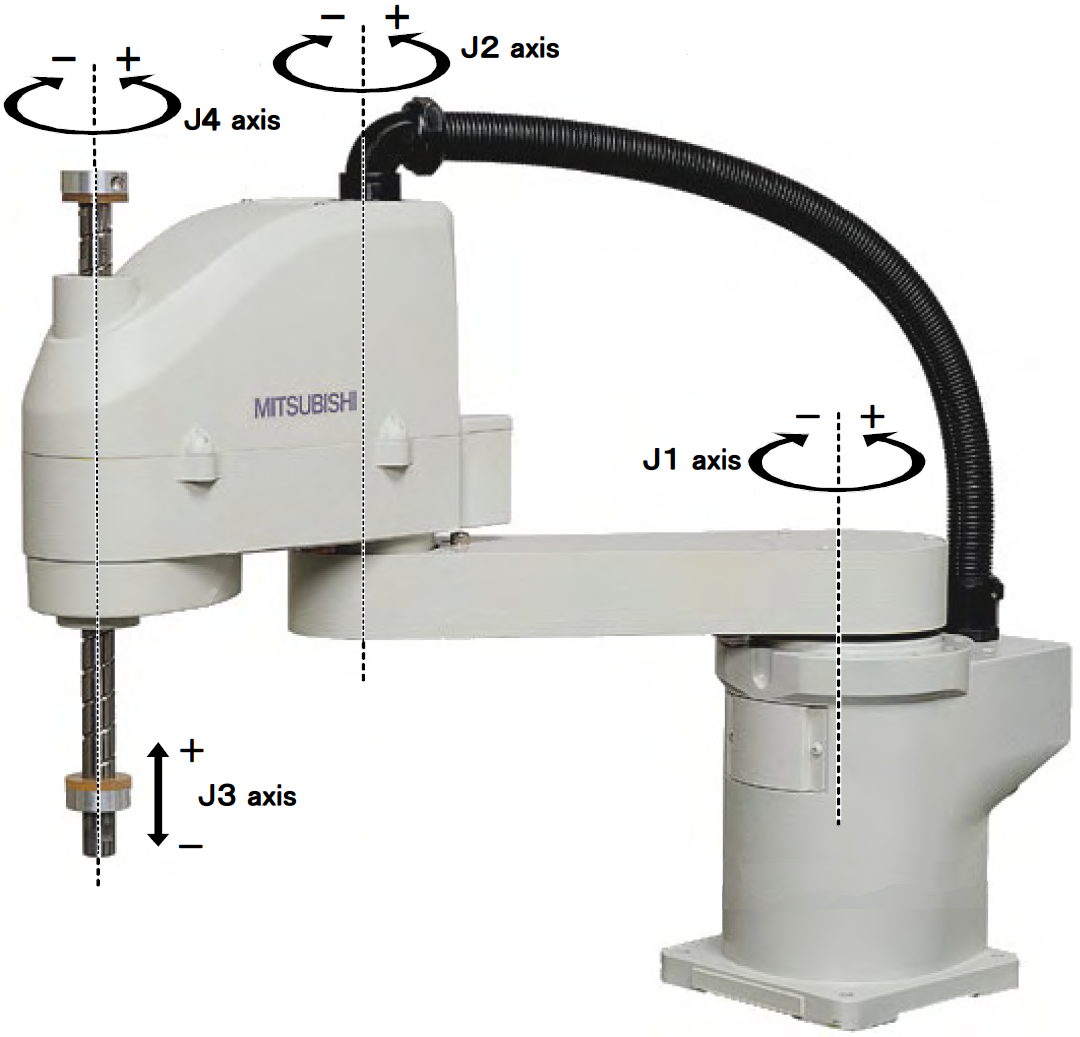
\includegraphics[width=\linewidth,height=.6\textheight,keepaspectratio]{../../figures/r22_scara.png}\\
\credit{SCARA robot. Mitsubishi Electric Automation, CC BY-SA 4.0, via Wikimedia Commons}
\end{columns}
\end{frame}

\begin{frame}[t]{Check your understanding (4.4)}
\begin{keybox}[Check your understanding]
\begin{enumerate}\small
\item Is the point $(0.6,\,0.5)$ m reachable by our arm ($L_1=0.4$, $L_2=0.3$ m)? Why?
\item For the target $(0.7,\,0)$ m, how many IK solutions are there? What are the joint angles?
\item A student computes $\theta_1$ with $\arctan(y/x)$ for a target at $(-0.3,\,-0.2)$ m. What goes wrong?
\end{enumerate}
\end{keybox}
\vspace{2mm}
\centering
\begin{tikzpicture}[scale=.5]
\fill[mkPale,even odd rule] (0,0) circle (2.8) (0,0) circle (.4);
\draw[mkMid] (0,0) circle (2.8); \draw[mkMid] (0,0) circle (.4);
\fill[mkOrange] (2.4,2.0) circle (3pt) node[right,lab] {1};
\fill[mkOrange] (2.8,0) circle (3pt) node[right,lab] {2};
\fill[mkOrange] (-1.2,-.8) circle (3pt) node[left,lab] {3};
\node[jnt] at (0,0) {};
\end{tikzpicture}
\end{frame}

\begin{frame}[t]{Session 4.4 summary and key terms}
\begin{columns}[T,onlytextwidth]
\column{.55\textwidth}
\begin{itemize}\small
\item IK: from desired tool position to joint angles
\item Reachable if $|L_1-L_2|\le r\le L_1+L_2$
\item $\theta_2$ from the law of cosines, $\theta_1$ from two \texttt{atan2}s
\item Two solutions (elbow up/down); a 6-axis arm has up to 8
\item Always check by plugging back into FK
\end{itemize}
\column{.41\textwidth}
\begin{defbox}[Key terms]
\small
\term{inverse kinematics}, \term{reachable workspace}, \term{atan2}, \term{configuration} (elbow up/down, lefty/righty), \term{spherical wrist}, \term{numerical IK}
\end{defbox}
\end{columns}
\end{frame}

% =====================================================================
\section{4.5 Velocity kinematics: the Jacobian}

\begin{frame}[t]{From joint speeds to tip speed}
\begin{columns}[T,onlytextwidth]
\column{.5\textwidth}
\begin{itemize}\small
\item Turn the shoulder at $\dot\theta_1$: the whole arm swings, tip moves \hl{perpendicular} to the line base--tip
\item Turn the elbow at $\dot\theta_2$: only link 2 swings
\item Tip speed = sum of the two contributions
\item Analogy: a door -- same rotation speed, the handle moves faster than a point near the hinge ($v=\omega r$)
\end{itemize}
\begin{notebox}
How fast the tip moves depends on the \emph{pose}, not only on the joint speeds.
\end{notebox}
\column{.46\textwidth}
\centering
\begin{tikzpicture}[scale=.9]
\draw[->,mkGray] (-.3,0) -- (4.2,0) node[right,lab] {$x$};
\draw[->,mkGray] (0,-.3) -- (0,3.6) node[above,lab] {$y$};
\arm{20}{70}{lnk}
\draw[mkGray,dashed] (0,0) -- (T);
\draw[vec,mkOrange] (T) -- ($(T)!1.3cm!90:(0,0)$) node[left,lab,text=mkOrange] {from $\dot\theta_1$};
\draw[vec,mkGreen] (T) -- ($(T)!1.0cm!90:(E)$) node[below left,lab,text=mkGreen] {from $\dot\theta_2$};
\draw[mkMid,->] (.7,-.1) arc (-10:40:.7) node[right,lab] {$\dot\theta_1$};
\base
\end{tikzpicture}
\end{columns}
\end{frame}

\begin{frame}[t]{Refresher: partial derivatives and matrix--vector products}
\begin{columns}[T,onlytextwidth]
\column{.5\textwidth}
\begin{defbox}[Refresher: partial derivative]
$\dfrac{\partial x}{\partial\theta_1}$: how much $x$ changes when \emph{only} $\theta_1$ changes (all other variables frozen).
\[ \dot x = \frac{\partial x}{\partial\theta_1}\dot\theta_1 + \frac{\partial x}{\partial\theta_2}\dot\theta_2 \]
(chain rule)
\end{defbox}
\column{.46\textwidth}
\begin{defbox}[Refresher: matrix times vector]
\[ \begin{bmatrix} a & b\\ c & d\end{bmatrix}\begin{bmatrix} u\\ w\end{bmatrix} = \begin{bmatrix} au+bw\\ cu+dw\end{bmatrix} \]
Each row: ``this much of $u$ plus this much of $w$''.
\end{defbox}
\begin{notebox}
Stacking the partial derivatives into a matrix gives the \term{Jacobian}.
\end{notebox}
\end{columns}
\end{frame}

\begin{frame}[t]{The Jacobian of the 2-link arm}
\begin{columns}[T,onlytextwidth]
\column{.56\textwidth}
\begin{itemize}\small
\item Differentiate the FK equations with respect to each joint angle
\end{itemize}
\begin{eqbox}
\[ \underbrace{\begin{bmatrix}\dot x\\ \dot y\end{bmatrix}}_{\bm v} =
\underbrace{\begin{bmatrix} -L_1 s_1 - L_2 s_{12} & -L_2 s_{12}\\ \phantom{-}L_1 c_1 + L_2 c_{12} & \phantom{-}L_2 c_{12}\end{bmatrix}}_{J(\bm\theta)}
\underbrace{\begin{bmatrix}\dot\theta_1\\ \dot\theta_2\end{bmatrix}}_{\dot{\bm\theta}} \]
\end{eqbox}
\begin{itemize}\small
\item Column 1: tip velocity per rad/s of joint 1; column 2: of joint 2
\item $J$ depends on the angles $\rightarrow$ it changes as the robot moves
\end{itemize}
\column{.4\textwidth}
\begin{keybox}[The Jacobian]
\small
\[ \bm v = J(\bm\theta)\,\dot{\bm\theta} \]
Units: \si{m/s} per \si{rad/s}, i.e.\ metres (a lever arm).\\[1mm]
For a 6-axis arm $J$ is $6\times6$: 3 linear + 3 angular velocities.
\end{keybox}
\end{columns}
\end{frame}

\begin{frame}[t]{Worked example: tip velocity}
\begin{columns}[T,onlytextwidth]
\column{.55\textwidth}
\small
Pose $\theta_1=0$, $\theta_2=\SI{90}{\degree}$ (tip at $(0.4,\,0.3)$ m).
\begin{enumerate}
\item $s_1=0$, $c_1=1$, $s_{12}=1$, $c_{12}=0$
\item $J=\begin{bmatrix} -0.3 & -0.3\\ 0.4 & 0\end{bmatrix}$ m
\item Shoulder only, $\dot\theta=(1,\,0)$ rad/s:\\ $\bm v=(-0.3,\;0.4)$ m/s, $|\bm v|=\SI{0.5}{m/s}$
\item Elbow only, $\dot\theta=(0,\,1)$ rad/s:\\ $\bm v=(-0.3,\;0)$ m/s, $|\bm v|=\SI{0.3}{m/s}$
\end{enumerate}
\begin{notebox}
Step 3: $|\bm v| = \omega\cdot r$ with $r=\SI{0.5}{m}$ (base-to-tip distance). The door rule again.
\end{notebox}
\column{.41\textwidth}
\centering
\begin{tikzpicture}[scale=.9]
\draw[->,mkGray] (-.3,0) -- (3.4,0) node[right,lab] {$x$};
\draw[->,mkGray] (0,-.3) -- (0,3.2) node[above,lab] {$y$};
\arm{0}{90}{lnk}
\draw[vec,mkOrange] (T) -- ++(-1.5,2.0) node[above,lab,text=mkOrange] {$(-0.3,0.4)$};
\draw[vec,mkGreen] (T) -- ++(-1.5,0) node[left,lab,text=mkGreen] {$(-0.3,0)$};
\node[lab,right] at (T) {$(0.4,0.3)$};
\base
\end{tikzpicture}
\end{columns}
\end{frame}

\begin{frame}[t]{Singularities: when the Jacobian loses a direction}
\begin{columns}[T,onlytextwidth]
\column{.48\textwidth}
\begin{itemize}\small
\item Determinant: $\det J = L_1L_2\sin\theta_2$
\item $\det J=0$ at $\theta_2=\SI{0}{\degree}$ (stretched) or $\SI{180}{\degree}$ (folded): a \term{singularity}
\item There the tip \hl{cannot move} along the arm (radially), whatever the joints do
\item Near it, a small tip speed needs \hl{huge} joint speeds: $\dot{\bm\theta}=J^{-1}\bm v$
\end{itemize}
\begin{notebox}
Analogy: with your arm fully stretched you cannot push your hand any further out.
\end{notebox}
\column{.48\textwidth}
\begin{tikzpicture}
\begin{axis}[mkplot,width=6.3cm,height=4.9cm,xmin=0,xmax=180,ymin=0,ymax=1.1,
  xlabel={elbow angle $\theta_2$ (\si{\degree})},ylabel={normalised value},xtick={0,45,90,135,180},
  legend pos=north east, legend cell align=left]
\addplot[mkBlue,thick,domain=0:180,samples=91] {sin(x)};
\addlegendentry{$\det J/(L_1L_2)$}
\addplot[mkOrange,thick,domain=5.7:174.3,samples=120] {0.1/sin(x)};
\addlegendentry{needed $\dot\theta$ (scaled)}
\end{axis}
\end{tikzpicture}
\end{columns}
\end{frame}

\begin{frame}[t]{Singularities of real 6-axis robots}
\begin{columns}[T,onlytextwidth]
\column{.56\textwidth}
\begin{itemize}\small
\item \term{Wrist singularity}: axes 4 and 6 line up (axis 5 at \SI{0}{\degree}) -- two motors fight for the same rotation
\item \term{Elbow singularity}: arm fully stretched (like our 2-link)
\item \term{Shoulder singularity}: wrist centre directly above axis 1
\item Effect: in a straight-line move the joints suddenly spin fast $\rightarrow$ the controller stops with an error
\item Fix: plan paths around them, or use a joint (PTP) move
\end{itemize}
\gofurther{Engineers measure ``distance from singularity'' with the \emph{manipulability} $\sqrt{\det(JJ^\mathsf{T})}$.}
\column{.4\textwidth}
\centering
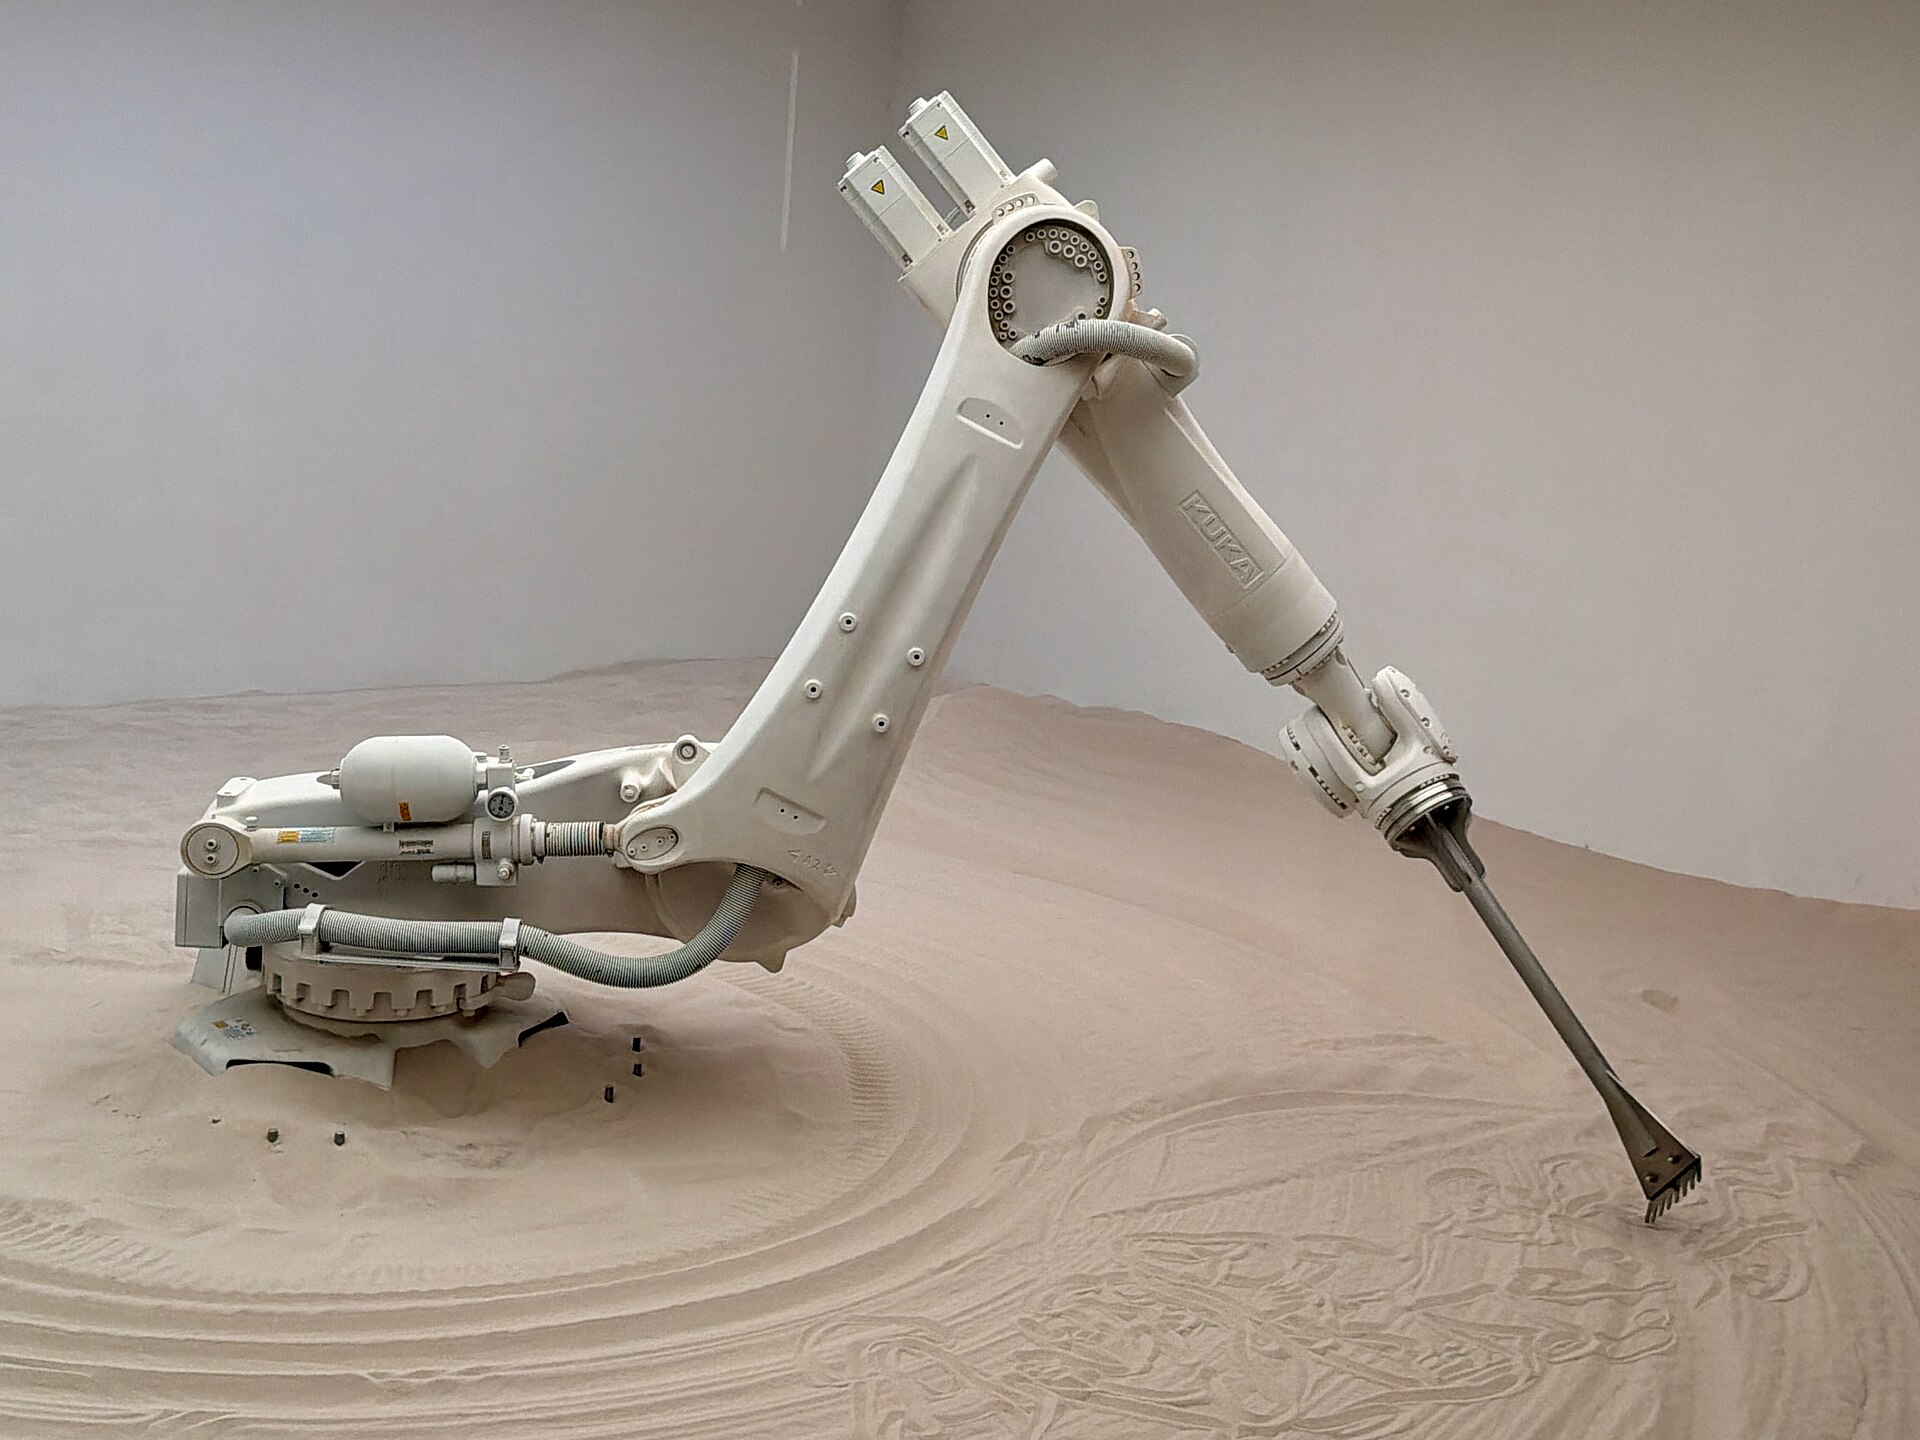
\includegraphics[width=\linewidth,height=.62\textheight,keepaspectratio]{../../figures/d4_kuka_robot.jpg}\\
\credit{KUKA industrial robot. Oleg Yunakov, CC BY-SA 4.0, via Wikimedia Commons}
\end{columns}
\end{frame}

\begin{frame}[t]{Statics: from tip force to joint torques}
\begin{columns}[T,onlytextwidth]
\column{.52\textwidth}
\begin{itemize}\small
\item The robot holds a load or presses on a surface: what torque must each motor give?
\item Power in = power out (no motion losses): $\bm\tau^\mathsf{T}\dot{\bm\theta}=\bm F^\mathsf{T}\bm v$
\item Insert $\bm v=J\dot{\bm\theta}$ and the same Jacobian appears, \hl{transposed}:
\end{itemize}
\begin{eqbox}
\[ \bm\tau = J^\mathsf{T}(\bm\theta)\,\bm F \]
\end{eqbox}
\begin{itemize}\small
\item $\bm F$ = force the tip exerts [N], $\bm\tau$ = joint torques [N\,m]
\end{itemize}
\column{.44\textwidth}
\centering
\begin{tikzpicture}[scale=.9]
\fill[pattern=north east lines,pattern color=mkGray] (3.7,-.2) rectangle (4.0,3.3);
\draw[mkGray,line width=.8pt] (3.7,-.2) -- (3.7,3.3);
\node[lab,rotate=90] at (4.2,1.6) {wall};
\arm{15}{60}{lnk}
\coordinate (W) at (T);
\draw[vec,mkOrange] (T) -- ++(1.0,0) node[above,lab,text=mkOrange] {$\bm F$};
\draw[mkMid,->,line width=.8pt] (-50:.55) arc (-50:60:.55);
\node[lab,text=mkMid] at (-.7,.2) {$\tau_1$};
\draw[mkMid,->,line width=.8pt] ($(E)+(-40:.45)$) arc (-40:90:.45);
\node[lab,text=mkMid] at ($(E)+(.6,-.3)$) {$\tau_2$};
\base
\end{tikzpicture}
\end{columns}
\end{frame}

\begin{frame}[t]{Worked example: holding a \SI{2}{kg} part}
\begin{columns}[T,onlytextwidth]
\column{.56\textwidth}
\small
Same pose as before: $\theta_1=0$, $\theta_2=\SI{90}{\degree}$. Links assumed massless.
\begin{enumerate}
\item Weight $\approx 2\times10=\SI{20}{N}$ down, so the tip must push \emph{up}: $\bm F=(0,\,20)$ N
\item $J^\mathsf{T}=\begin{bmatrix} -0.3 & 0.4\\ -0.3 & 0\end{bmatrix}$ m
\item $\tau_1=-0.3\cdot0+0.4\cdot20=\SI{8}{N.m}$
\item $\tau_2=-0.3\cdot0+0\cdot20=\SI{0}{N.m}$
\end{enumerate}
\begin{keybox}[Does it make sense?]
Joint 1: lever arm \SI{0.4}{m} $\times$ \SI{20}{N} $=$ \SI{8}{N.m} \checkmark.
Joint 2: link 2 is vertical, the force passes through the joint, no lever arm \checkmark.
\end{keybox}
\column{.4\textwidth}
\centering
\begin{tikzpicture}[scale=.9]
\draw[->,mkGray] (-.3,0) -- (3.2,0) node[right,lab] {$x$};
\arm{0}{90}{lnk}
\draw[mkOrange,fill=mkCream] ($(T)+(-.25,.05)$) rectangle ++(.5,.4);
\node[lab] at ($(T)+(0,.25)$) {\tiny 2kg};
\draw[vec,mkRed] ($(T)+(.45,.25)$) -- ++(0,-1.0) node[right,lab,text=mkRed] {$mg$};
\draw[vec,mkOrange] ($(T)+(-.5,-1.2)$) -- ++(0,1.0) node[left,lab,text=mkOrange] {$\bm F$};
\draw[mkGray,<->] (0,-.5) -- (2.4,-.5) node[midway,below,lab] {$\SI{0.4}{m}$};
\base
\end{tikzpicture}
\end{columns}
\end{frame}

\begin{frame}[t]{Check your understanding (4.5)}
\begin{columns}[T,onlytextwidth]
\column{.6\textwidth}
\begin{keybox}[Check your understanding]
\begin{enumerate}\small
\item In the pose $\theta_1=0$, $\theta_2=\SI{90}{\degree}$ the tip pushes on a wall with $\bm F=(10,\,0)$ N. Compute $\tau_1$ and $\tau_2$.
\item Why does a robot moving in a straight line through a stretched-arm pose stop with an error?
\item At a singularity, is it easy or hard for the robot to \emph{resist} a force along the arm? Think of standing with straight knees.
\end{enumerate}
\end{keybox}
\column{.36\textwidth}
\centering
\begin{tikzpicture}[scale=.8]
\arm{0}{90}{lnk}
\draw[vec,mkOrange] (T) -- ++(1.1,0) node[right,lab] {$10$ N};
\fill[pattern=north east lines,pattern color=mkGray] ($(T)+(1.6,-1)$) rectangle ++(.3,2);
\base
\end{tikzpicture}
\end{columns}
\end{frame}

\begin{frame}[t]{Session 4.5 summary and key terms}
\begin{columns}[T,onlytextwidth]
\column{.55\textwidth}
\begin{itemize}\small
\item Jacobian $J(\bm\theta)$: joint speeds $\rightarrow$ tip velocity, $\bm v=J\dot{\bm\theta}$
\item $J$ changes with the pose
\item Singularity: $\det J=0$, a tip direction is lost, joint speeds explode nearby
\item Same matrix for forces: $\bm\tau=J^\mathsf{T}\bm F$
\item Used for motor sizing, force control and numerical IK
\end{itemize}
\column{.41\textwidth}
\begin{defbox}[Key terms]
\small
\term{Jacobian}, \term{velocity kinematics}, \term{determinant}, \term{singularity} (wrist / elbow / shoulder), \term{manipulability}, \term{statics}, \term{virtual work}
\end{defbox}
\end{columns}
\end{frame}

% =====================================================================
\section{4.6 Introduction to robot dynamics}

\begin{frame}[t]{Why dynamics? Geometry is not enough}
\begin{columns}[T,onlytextwidth]
\column{.52\textwidth}
\begin{itemize}\small
\item Kinematics: \emph{where} and \emph{how fast} (geometry only)
\item Dynamics: \emph{which torques} are needed to make that motion happen
\item Analogy: carrying a full bucket with your arm stretched out vs.\ close to your body -- same bucket, very different effort
\item Needed for: motor sizing (W1D2), feedforward and computed-torque control (W1D4), simulation
\end{itemize}
\column{.44\textwidth}
\centering
\begin{tikzpicture}[node distance=7mm]
\node[blk,minimum width=34mm] (k) {Kinematics\\ $\bm\theta,\ \dot{\bm\theta},\ \ddot{\bm\theta}$};
\node[blko,minimum width=34mm,below=of k] (d) {Dynamics model\\ masses, inertias, gravity};
\node[blk,minimum width=34mm,below=of d] (t) {Joint torques $\bm\tau$\\ $\rightarrow$ motor currents};
\draw[sig] (k) -- (d); \draw[sig] (d) -- (t);
\end{tikzpicture}
\end{columns}
\end{frame}

\begin{frame}[t]{Refresher: rotation, energy and the Lagrange idea}
\begin{columns}[T,onlytextwidth]
\column{.5\textwidth}
\begin{defbox}[Refresher: Newton for rotation]
$\tau = J\alpha$: torque [N\,m] = inertia [\si{kg.m^2}] $\times$ angular acceleration [\si{rad/s^2}].
Point mass at radius $r$: $J=mr^2$.
\end{defbox}
\begin{defbox}[Refresher: energy]
Kinetic $K=\tfrac12 mv^2$, potential $P=mgh$.
\end{defbox}
\column{.46\textwidth}
\begin{keybox}[Lagrange in one sentence]
Write the total kinetic energy $K$ and potential energy $P$ of the arm; a standard recipe (differentiate $K-P$) gives the torque each joint needs.
\end{keybox}
\gofurther{The recipe is $\tau_i=\frac{d}{dt}\frac{\partial L}{\partial\dot\theta_i}-\frac{\partial L}{\partial\theta_i}$ with $L=K-P$. Robot software uses the faster Newton--Euler recursion.}
\end{columns}
\end{frame}

\begin{frame}[t]{The robot equation of motion}
\begin{eqbox}
\[ \bm\tau \;=\; \underbrace{M(\bm\theta)\,\ddot{\bm\theta}}_{\text{inertia}} \;+\; \underbrace{C(\bm\theta,\dot{\bm\theta})\,\dot{\bm\theta}}_{\text{Coriolis \& centrifugal}} \;+\; \underbrace{\bm g(\bm\theta)}_{\text{gravity}} \;\;(+\;\text{friction})\]
\end{eqbox}
\vspace{1mm}
\begin{columns}[T,onlytextwidth]
\column{.32\textwidth}
\begin{defbox}[Inertia term]
\small $M$: like $J$ in $\tau=J\alpha$, but a matrix that \hl{changes with the pose}.
\end{defbox}
\column{.32\textwidth}
\begin{defbox}[Velocity term]
\small Forces that appear because links rotate; grow with speed squared. Small at low speed.
\end{defbox}
\column{.32\textwidth}
\begin{defbox}[Gravity term]
\small Torque just to \hl{hold} the pose. Present even at standstill.
\end{defbox}
\end{columns}
\vspace{1mm}
\begin{notebox}
Same structure as a mass--spring--damper (W1D2): ``mass $\times$ acceleration + velocity term + position term = force''.
\end{notebox}
\end{frame}

\begin{frame}[t]{Gravity torque of the 2-link arm}
\begin{columns}[T,onlytextwidth]
\column{.48\textwidth}
\begin{itemize}\small
\item Simple model: point masses $m_1$ at the elbow, $m_2$ at the tip (link 2 + payload)
\item Torque = weight $\times$ horizontal lever arm
\end{itemize}
\begin{eqbox}
\small
\[ \begin{aligned}
g_2 &= m_2\,g\,L_2\cos(\theta_1+\theta_2)\\
g_1 &= (m_1+m_2)\,g\,L_1\cos\theta_1 + g_2
\end{aligned}\]
\end{eqbox}
\begin{itemize}\small
\item Maximum when the arm is \hl{horizontal}, zero when vertical
\end{itemize}
\column{.48\textwidth}
\begin{tikzpicture}
\begin{axis}[mkplot,width=6.3cm,height=4.8cm,xmin=-90,xmax=90,ymin=-30,ymax=30,
  xlabel={shoulder angle $\theta_1$ (\si{\degree}), with $\theta_2=0$},ylabel={torque (\si{N.m})},xtick={-90,-45,0,45,90},
  legend pos=south east,legend cell align=left]
\addplot[mkBlue,thick,domain=-90:90,samples=61] {26*cos(x)};
\addlegendentry{$g_1$ shoulder}
\addplot[mkOrange,thick,domain=-90:90,samples=61] {6*cos(x)};
\addlegendentry{$g_2$ elbow}
\end{axis}
\end{tikzpicture}\\
{\scriptsize $m_1=\SI{3}{kg}$, $m_2=\SI{2}{kg}$, $g\approx\SI{10}{m/s^2}$}
\end{columns}
\end{frame}

\begin{frame}[t]{Worked example: holding the arm horizontal}
\begin{columns}[T,onlytextwidth]
\column{.55\textwidth}
\small
$m_1=\SI{3}{kg}$, $m_2=\SI{2}{kg}$, $L_1=\SI{0.4}{m}$, $L_2=\SI{0.3}{m}$, $\theta_1=\theta_2=0$.
\begin{enumerate}
\item Elbow: $g_2=2\cdot10\cdot0.3=\SI{6}{N.m}$
\item Shoulder, own part: $(3+2)\cdot10\cdot0.4=\SI{20}{N.m}$
\item Shoulder total: $g_1=20+6=\SI{26}{N.m}$
\item Add a \SI{1}{kg} payload ($m_2=\SI{3}{kg}$): $g_2=\SI{9}{N.m}$, $g_1=24+9=\SI{33}{N.m}$
\end{enumerate}
\begin{keybox}[Take-away]
\SI{1}{kg} more payload costs \SI{7}{N.m} at the shoulder: the lever arm is the whole reach (\SI{0.7}{m}).
\end{keybox}
\column{.41\textwidth}
\centering
\begin{tikzpicture}[scale=.9]
\arm{0}{0}{lnk}
\fill[mkMid] (E) circle (4pt) node[above=2pt,lab] {$m_1$};
\fill[mkOrange] (T) circle (4pt) node[above=2pt,lab] {$m_2$};
\draw[vec,mkRed] (E) -- ++(0,-1) node[below,lab] {$m_1g$};
\draw[vec,mkRed] (T) -- ++(0,-1) node[below,lab] {$m_2g$};
\draw[mkGray,<->] (0,.6) -- (2.4,.6) node[midway,above,lab] {0.4 m};
\draw[mkGray,<->] (2.4,.6) -- (4.2,.6) node[midway,above,lab] {0.3 m};
\base
\end{tikzpicture}
\end{columns}
\end{frame}

\begin{frame}[t]{Inertia changes with the pose}
\begin{columns}[T,onlytextwidth]
\column{.48\textwidth}
\begin{itemize}\small
\item Inertia seen by the shoulder (point masses):
\end{itemize}
\begin{eqbox}
\small
\[ M_{11} = m_1L_1^2 + m_2\big(L_1^2+L_2^2+2L_1L_2\cos\theta_2\big) \]
\end{eqbox}
\begin{itemize}\small
\item Stretched ($\theta_2=0$): $0.48+2\cdot0.49=\SI{1.46}{kg.m^2}$
\item Folded ($\theta_2=\SI{180}{\degree}$): $0.48+2\cdot0.01=\SI{0.50}{kg.m^2}$
\item Factor $\approx 3$ $\rightarrow$ a fixed PID tuning behaves differently in different poses
\end{itemize}
\begin{notebox}Analogy: a figure skater pulls in the arms and spins faster.\end{notebox}
\column{.48\textwidth}
\begin{tikzpicture}
\begin{axis}[mkplot,width=6.3cm,height=4.8cm,xmin=0,xmax=180,ymin=0,ymax=2.2,
  xlabel={elbow angle $\theta_2$ (\si{\degree})},ylabel={$M_{11}$ (\si{kg.m^2})},xtick={0,45,90,135,180},
  legend pos=north east,legend cell align=left]
\addplot[mkBlue,thick,domain=0:180,samples=61] {0.48+2*(0.25+0.24*cos(x))};
\addlegendentry{$m_2=2$ kg}
\addplot[mkOrange,thick,domain=0:180,samples=61] {0.48+3*(0.25+0.24*cos(x))};
\addlegendentry{$m_2=3$ kg (payload)}
\end{axis}
\end{tikzpicture}
\end{columns}
\end{frame}

\begin{frame}[t]{Payload effects and Coriolis forces}
\begin{columns}[T,onlytextwidth]
\column{.5\textwidth}
\textbf{\small Payload}
\begin{itemize}\small
\item More payload $\rightarrow$ more gravity torque \emph{and} more inertia
\item Datasheet payload (e.g.\ \SI{10}{kg}) is valid only at a given distance from the flange
\item Robot controllers ask for payload mass and centre of gravity: wrong data $\rightarrow$ overshoot, path errors, false collision alarms
\end{itemize}
\column{.46\textwidth}
\textbf{\small Coriolis and centrifugal}
\begin{itemize}\small
\item Analogy: walking outward on a turning merry-go-round, you are pushed sideways
\item Grow with $\dot\theta^2$: unimportant when slow, large for fast pick-and-place
\end{itemize}
\gofurther{\emph{Computed-torque control} (W1D4) uses $M$, $C$, $\bm g$ to cancel the robot's own dynamics; delta robots reach $>\SI{100}{m/s^2}$ partly because their moving mass is so small.}
\end{columns}
\end{frame}

\begin{frame}[t]{Worked example: torque to accelerate the shoulder}
\begin{columns}[T,onlytextwidth]
\column{.52\textwidth}
\small
Arm stretched and horizontal, start moving up with $\ddot\theta_1=\SI{10}{rad/s^2}$ (from rest, so no Coriolis term).
\begin{enumerate}
\item $\tau_1 = M_{11}\,\ddot\theta_1 + g_1$
\item No payload: $1.46\cdot10+26=14.6+26=\SI{40.6}{N.m}$
\item \SI{1}{kg} payload: $M_{11}=0.48+3\cdot0.49=\SI{1.95}{kg.m^2}$\\
$\tau_1=19.5+33=\SI{52.5}{N.m}$
\end{enumerate}
\begin{keybox}[Take-away]
Gravity is the larger part here; payload adds about 30\,\% torque.
\end{keybox}
\column{.44\textwidth}
\begin{tikzpicture}
\begin{axis}[mkplot,ybar stacked,width=6cm,height=4.8cm,ymin=0,ymax=60,bar width=14mm,
  symbolic x coords={no payload,1 kg payload},xtick=data,ylabel={$\tau_1$ (\si{N.m})},
  legend pos=north west,legend cell align=left,enlarge x limits=.5,
  nodes near coords,every node near coord/.append style={font=\tiny}]
\addplot[fill=mkOrange,draw=mkOrange] coordinates {(no payload,26) (1 kg payload,33)};
\addlegendentry{gravity}
\addplot[fill=mkSky,draw=mkMid] coordinates {(no payload,14.6) (1 kg payload,19.5)};
\addlegendentry{inertia}
\end{axis}
\end{tikzpicture}
\end{columns}
\end{frame}

\begin{frame}[t]{Check your understanding (4.6)}
\begin{keybox}[Check your understanding]
\begin{enumerate}\small
\item The arm points straight up ($\theta_1=\SI{90}{\degree}$, $\theta_2=0$). What are the gravity torques $g_1$ and $g_2$?
\item Why does a robot axis need more torque to accelerate when the arm is stretched than when it is folded?
\item Which term of the equation of motion can you ignore for a slow painting robot, and which never?
\end{enumerate}
\end{keybox}
\end{frame}

\begin{frame}[t]{Session 4.6 summary and key terms}
\begin{columns}[T,onlytextwidth]
\column{.55\textwidth}
\begin{itemize}\small
\item $\bm\tau=M(\bm\theta)\ddot{\bm\theta}+C\dot{\bm\theta}+\bm g(\bm\theta)$
\item Gravity: holding torque, largest with the arm horizontal
\item Inertia depends on the pose (factor 3 in our arm)
\item Payload raises both gravity and inertia torques
\item Coriolis/centrifugal matter only at high speed
\end{itemize}
\column{.41\textwidth}
\begin{defbox}[Key terms]
\small
\term{dynamics}, \term{Lagrangian}, \term{inertia (mass) matrix}, \term{gravity torque}, \term{Coriolis / centrifugal}, \term{payload}, \term{computed torque}
\end{defbox}
\end{columns}
\end{frame}

% =====================================================================
\section{4.7 Motion systems and trajectory planning}

\begin{frame}[t]{Path and trajectory}
\begin{columns}[T,onlytextwidth]
\column{.52\textwidth}
\begin{itemize}\small
\item \term{Path}: the geometric curve the tool follows (\emph{where})
\item \term{Trajectory}: path + timing: position, velocity, acceleration at each instant (\emph{where and when})
\item Analogy: a route on a map vs.\ a train timetable
\item The planner sends new set-points to every axis each \term{interpolation cycle} (typically 1--4 ms)
\end{itemize}
\column{.44\textwidth}
\centering
\begin{tikzpicture}[node distance=5mm]
\node[blk,minimum width=36mm] (p) {Program: targets, speed};
\node[blko,minimum width=36mm,below=of p] (i) {Trajectory planner\\(interpolator)};
\node[blk,minimum width=36mm,below=of i] (k) {IK (if Cartesian)};
\node[blk,minimum width=36mm,below=of k] (s) {Servo loops (W1D5)};
\draw[sig] (p) -- (i); \draw[sig] (i) -- (k); \draw[sig] (k) -- (s);
\node[lab,right=1mm of k,text=mkGray] {every 1--4 ms};
\end{tikzpicture}
\end{columns}
\end{frame}

\begin{frame}[t]{Point-to-point (PTP) moves in joint space}
\begin{columns}[T,onlytextwidth]
\column{.45\textwidth}
\begin{itemize}\small
\item Interpolate each \hl{joint angle} from start to end
\item All joints start and stop together (\term{synchronised PTP})
\item Fastest move, no IK along the way, no singularity trouble
\item But the tool path is a \hl{curve}, not easy to predict
\item Used for free moves through the air
\end{itemize}
\column{.52\textwidth}
\begin{tikzpicture}
\begin{axis}[mkplot,width=6.6cm,height=5.2cm,axis equal image,xmin=-0.35,xmax=0.75,ymin=-0.05,ymax=0.65,
  xlabel={$x$ (m)},ylabel={$y$ (m)},legend pos=south west,legend cell align=left]
\addplot[mkOrange,thick,domain=0:1,samples=41,variable=\t]
  ({0.4*cos(2.48+73.97*t)+0.3*cos(70.46+97.78*t)},{0.4*sin(2.48+73.97*t)+0.3*sin(70.46+97.78*t)});
\addlegendentry{PTP (joint interpolation)}
\addplot[mkBlue,thick,dashed] coordinates {(0.5,0.3) (-0.2,0.45)};
\addlegendentry{LIN (straight line)}
\addplot[only marks,mark=*,mkNavy,mark size=1.5pt] coordinates {(0.5,0.3) (-0.2,0.45)};
\node[font=\tiny,anchor=west] at (axis cs:0.5,0.27) {A};
\node[font=\tiny,anchor=east] at (axis cs:-0.2,0.42) {B};
\addplot[mkGray,thin,domain=0:180,samples=40] ({0.7*cos(x)},{0.7*sin(x)});
\end{axis}
\end{tikzpicture}
\end{columns}
\end{frame}

\begin{frame}[t]{Velocity profiles: trapezoid and S-curve}
\begin{columns}[T,onlytextwidth]
\column{.45\textwidth}
\begin{itemize}\small
\item Recap W1D5: accelerate, cruise, decelerate
\item \term{Trapezoidal} profile: limited velocity and acceleration
\item \term{S-curve}: also limits \term{jerk} (rate of change of acceleration) $\rightarrow$ less shaking
\end{itemize}
\begin{keybox}[Worked example]
\small
$\Delta\theta=\SI{90}{\degree}$, $\omega_{\max}=\SI{180}{\degree/s}$, $\alpha=\SI{720}{\degree/s^2}$
\begin{enumerate}
\item $t_a=180/720=\SI{0.25}{s}$, angle $\tfrac12\cdot720\cdot0.25^2=\SI{22.5}{\degree}$
\item Accel + decel: \SI{45}{\degree}; cruise \SI{45}{\degree} in \SI{0.25}{s}
\item Total: $0.25+0.25+0.25=\SI{0.75}{s}$
\end{enumerate}
\end{keybox}
\column{.52\textwidth}
\begin{tikzpicture}
\begin{axis}[mkplot,width=6.6cm,height=4.8cm,xmin=0,xmax=0.8,ymin=0,ymax=210,
  xlabel={time (s)},ylabel={joint speed (\si{\degree/s})},legend pos=north east,legend cell align=left]
\addplot[mkBlue,thick] coordinates {(0,0) (0.25,180) (0.5,180) (0.75,0)};
\addlegendentry{trapezoid}
\addplot[mkOrange,thick,domain=0:0.25,samples=30] {90*(1-cos(720*x))};
\addlegendentry{S-curve (smoothed)}
\addplot[mkOrange,thick,forget plot] coordinates {(0.25,180) (0.5,180)};
\addplot[mkOrange,thick,domain=0.5:0.75,samples=30,forget plot] {90*(1+cos(720*(x-0.5)))};
\end{axis}
\end{tikzpicture}\\
{\scriptsize The S-curve here (sine-shaped acceleration) has the same duration but peak acceleration $\approx 1.6\times$ higher.}
\end{columns}
\end{frame}

\begin{frame}[t]{Linear (LIN) and circular (CIRC) moves in Cartesian space}
\begin{columns}[T,onlytextwidth]
\column{.5\textwidth}
\begin{itemize}\small
\item \term{LIN}: tool centre point (TCP) moves on a straight line with constant orientation change
\item \term{CIRC}: arc through a \hl{via point} to the end point
\item Planner cuts the path into small steps and runs \hl{IK at every step}
\item Needed for welding, gluing, insertion, cutting
\item Risk: passing near a singularity $\rightarrow$ joint speed limit error
\item \term{Blending} (fly-by): round the corners between moves to avoid stopping
\end{itemize}
\column{.46\textwidth}
\centering
\begin{tikzpicture}[scale=.95]
\draw[mkBlue,line width=1.2pt] (0,0) -- (2.4,0);
\draw[mkBlue,line width=1.2pt] (2.4,0) .. controls (3.0,0) and (3.2,.3) .. (3.2,.8);
\draw[mkOrange,line width=1.2pt] (3.2,.8) arc (0:150:1.6);
\foreach \p/\n in {(0,0)/P1,(3.2,.8)/P2} \fill[mkNavy] \p circle (2pt) node[below,lab] {\n};
\fill[mkNavy] (1.6,2.4) circle (2pt) node[above,lab] {via};
\draw[mkGray,dashed] (2.4,0) -- (3.2,0) -- (3.2,.8);
\node[lab,text=mkBlue] at (1.2,-.35) {LIN};
\node[lab,text=mkOrange] at (2.9,2.1) {CIRC};
\node[lab,text=mkGray,align=left] at (3.9,-.35) {blend zone};
\foreach \s in {0,.3,...,2.4} \draw[mkSky] (\s,-.08) -- (\s,.08);
\node[lab,text=mkGray] at (1.2,.35) {IK at each tick};
\end{tikzpicture}
\end{columns}
\end{frame}

\begin{frame}[t]{Joint space vs.\ Cartesian space: when to use which}
\centering
\small
\begin{tabularx}{.92\textwidth}{@{}l X X@{}}
\toprule
 & \textbf{Joint space (PTP)} & \textbf{Cartesian space (LIN / CIRC)}\\
\midrule
Tool path & curved, depends on robot & straight line or arc, predictable\\
Speed & fastest (each joint near its limit) & limited by the slowest joint along the path\\
Computation & interpolate angles only & IK every cycle\\
Singularities & no problem & can stop the move\\
Configuration & may change (elbow flips) & must stay the same\\
Typical use & approach, free transfer, retract & process path: weld, glue, insert\\
\bottomrule
\end{tabularx}
\vspace{3mm}
\begin{notebox}
Rule of thumb: \textbf{PTP through the air, LIN near the part.} A typical pick: PTP to above the part, LIN down, grip, LIN up, PTP away.
\end{notebox}
\end{frame}

\begin{frame}[t]{Linear axes and gantries: the easy kinematics}
\begin{columns}[T,onlytextwidth]
\column{.52\textwidth}
\begin{itemize}\small
\item \term{Cartesian / gantry robot}: three prismatic axes along $x$, $y$, $z$
\item FK and IK are trivial: $x=q_1$, $y=q_2$, $z=q_3$; no singularities
\item Drives: ball screw, belt, rack-and-pinion or linear motor (W1D2)
\item Large, stiff, accurate: CNC loading, 3D printers, palletising over long distances
\item Often a \term{7th axis}: a linear track carrying an articulated robot
\end{itemize}
\column{.44\textwidth}
\centering
\begin{tikzpicture}[scale=.85]
\draw[mkGray,fill=mkLight] (0,0) rectangle (.25,2.6); \draw[mkGray,fill=mkLight] (4,0) rectangle (4.25,2.6);
\draw[mkBlue,fill=mkPale,line width=.8pt] (0,2.6) rectangle (4.25,2.9);
\node[lab] at (2.1,3.15) {$x$ axis (beam)};
\draw[mkOrange,fill=mkCream,line width=.8pt] (1.8,2.25) rectangle (2.6,2.6);
\draw[mkOrange,line width=2.5pt] (2.2,2.25) -- (2.2,1.0);
\node[lab,right] at (2.3,1.6) {$z$ axis};
\draw[mkNavy,line width=1pt] (1.95,1.0) -- (2.45,1.0) (1.95,1.0) -- (1.95,.75) (2.45,1.0) -- (2.45,.75);
\draw[vec,mkMid] (2.8,2.42) -- (3.6,2.42);
\draw[mkGray] (-.3,0) -- (4.6,0);
\draw[mkGray,fill=mkCream] (1.7,0) rectangle (2.7,.4);
\node[lab] at (2.2,-.3) {part};
\end{tikzpicture}
\end{columns}
\end{frame}

\begin{frame}[t]{Differential-drive mobile robots (AMRs)}
\begin{columns}[T,onlytextwidth]
\column{.52\textwidth}
\begin{itemize}\small
\item Two driven wheels (radius $r$) on one axle, track width $b$, plus caster wheels
\item Same wheel speeds: straight; different: turn; opposite: spin on the spot
\end{itemize}
\begin{eqbox}
\[ v=\frac{r(\omega_R+\omega_L)}{2},\qquad \omega=\frac{r(\omega_R-\omega_L)}{b} \]
\end{eqbox}
\begin{itemize}\small
\item Cannot move sideways (\term{nonholonomic}) -- like a shopping trolley with fixed rear wheels
\end{itemize}
\column{.44\textwidth}
\centering
\begin{tikzpicture}[scale=.9]
\draw[mkBlue,fill=mkPale,line width=.8pt,rounded corners=3pt] (-1.2,-1) rectangle (1.2,1.2);
\fill[mkNavy] (-1.45,-.45) rectangle (-1.2,.45); \fill[mkNavy] (1.2,-.45) rectangle (1.45,.45);
\draw[mkGray,dashed] (-1.6,0) -- (1.6,0);
\draw[mkGray,<->] (-1.32,-1.3) -- (1.32,-1.3) node[midway,below,lab] {$b$};
\draw[vec,mkOrange] (0,0) -- (0,1.7) node[above,lab] {$v$};
\draw[mkMid,->,line width=.8pt] (.5,0) arc (0:120:.5) node[left,lab] {$\omega$};
\draw[vec,mkGreen] (1.6,0) -- (1.6,1.1) node[right,lab] {$r\omega_R$};
\draw[vec,mkGreen] (-1.6,0) -- (-1.6,.8) node[left,lab] {$r\omega_L$};
\fill[mkNavy] (0,0) circle (1.5pt);
\end{tikzpicture}
\end{columns}
\end{frame}

\begin{frame}[t]{Worked example: an AMR turning in a warehouse}
\begin{columns}[T,onlytextwidth]
\column{.5\textwidth}
\small
$r=\SI{0.1}{m}$, $b=\SI{0.5}{m}$, $\omega_R=\SI{10}{rad/s}$, $\omega_L=\SI{8}{rad/s}$.
\begin{enumerate}
\item $v=0.1\cdot(10+8)/2=\SI{0.9}{m/s}$
\item $\omega=0.1\cdot(10-8)/0.5=\SI{0.4}{rad/s}$
\item Turning radius $R=v/\omega=\SI{2.25}{m}$
\item Quarter circle takes $(\pi/2)/0.4\approx\SI{3.9}{s}$
\end{enumerate}
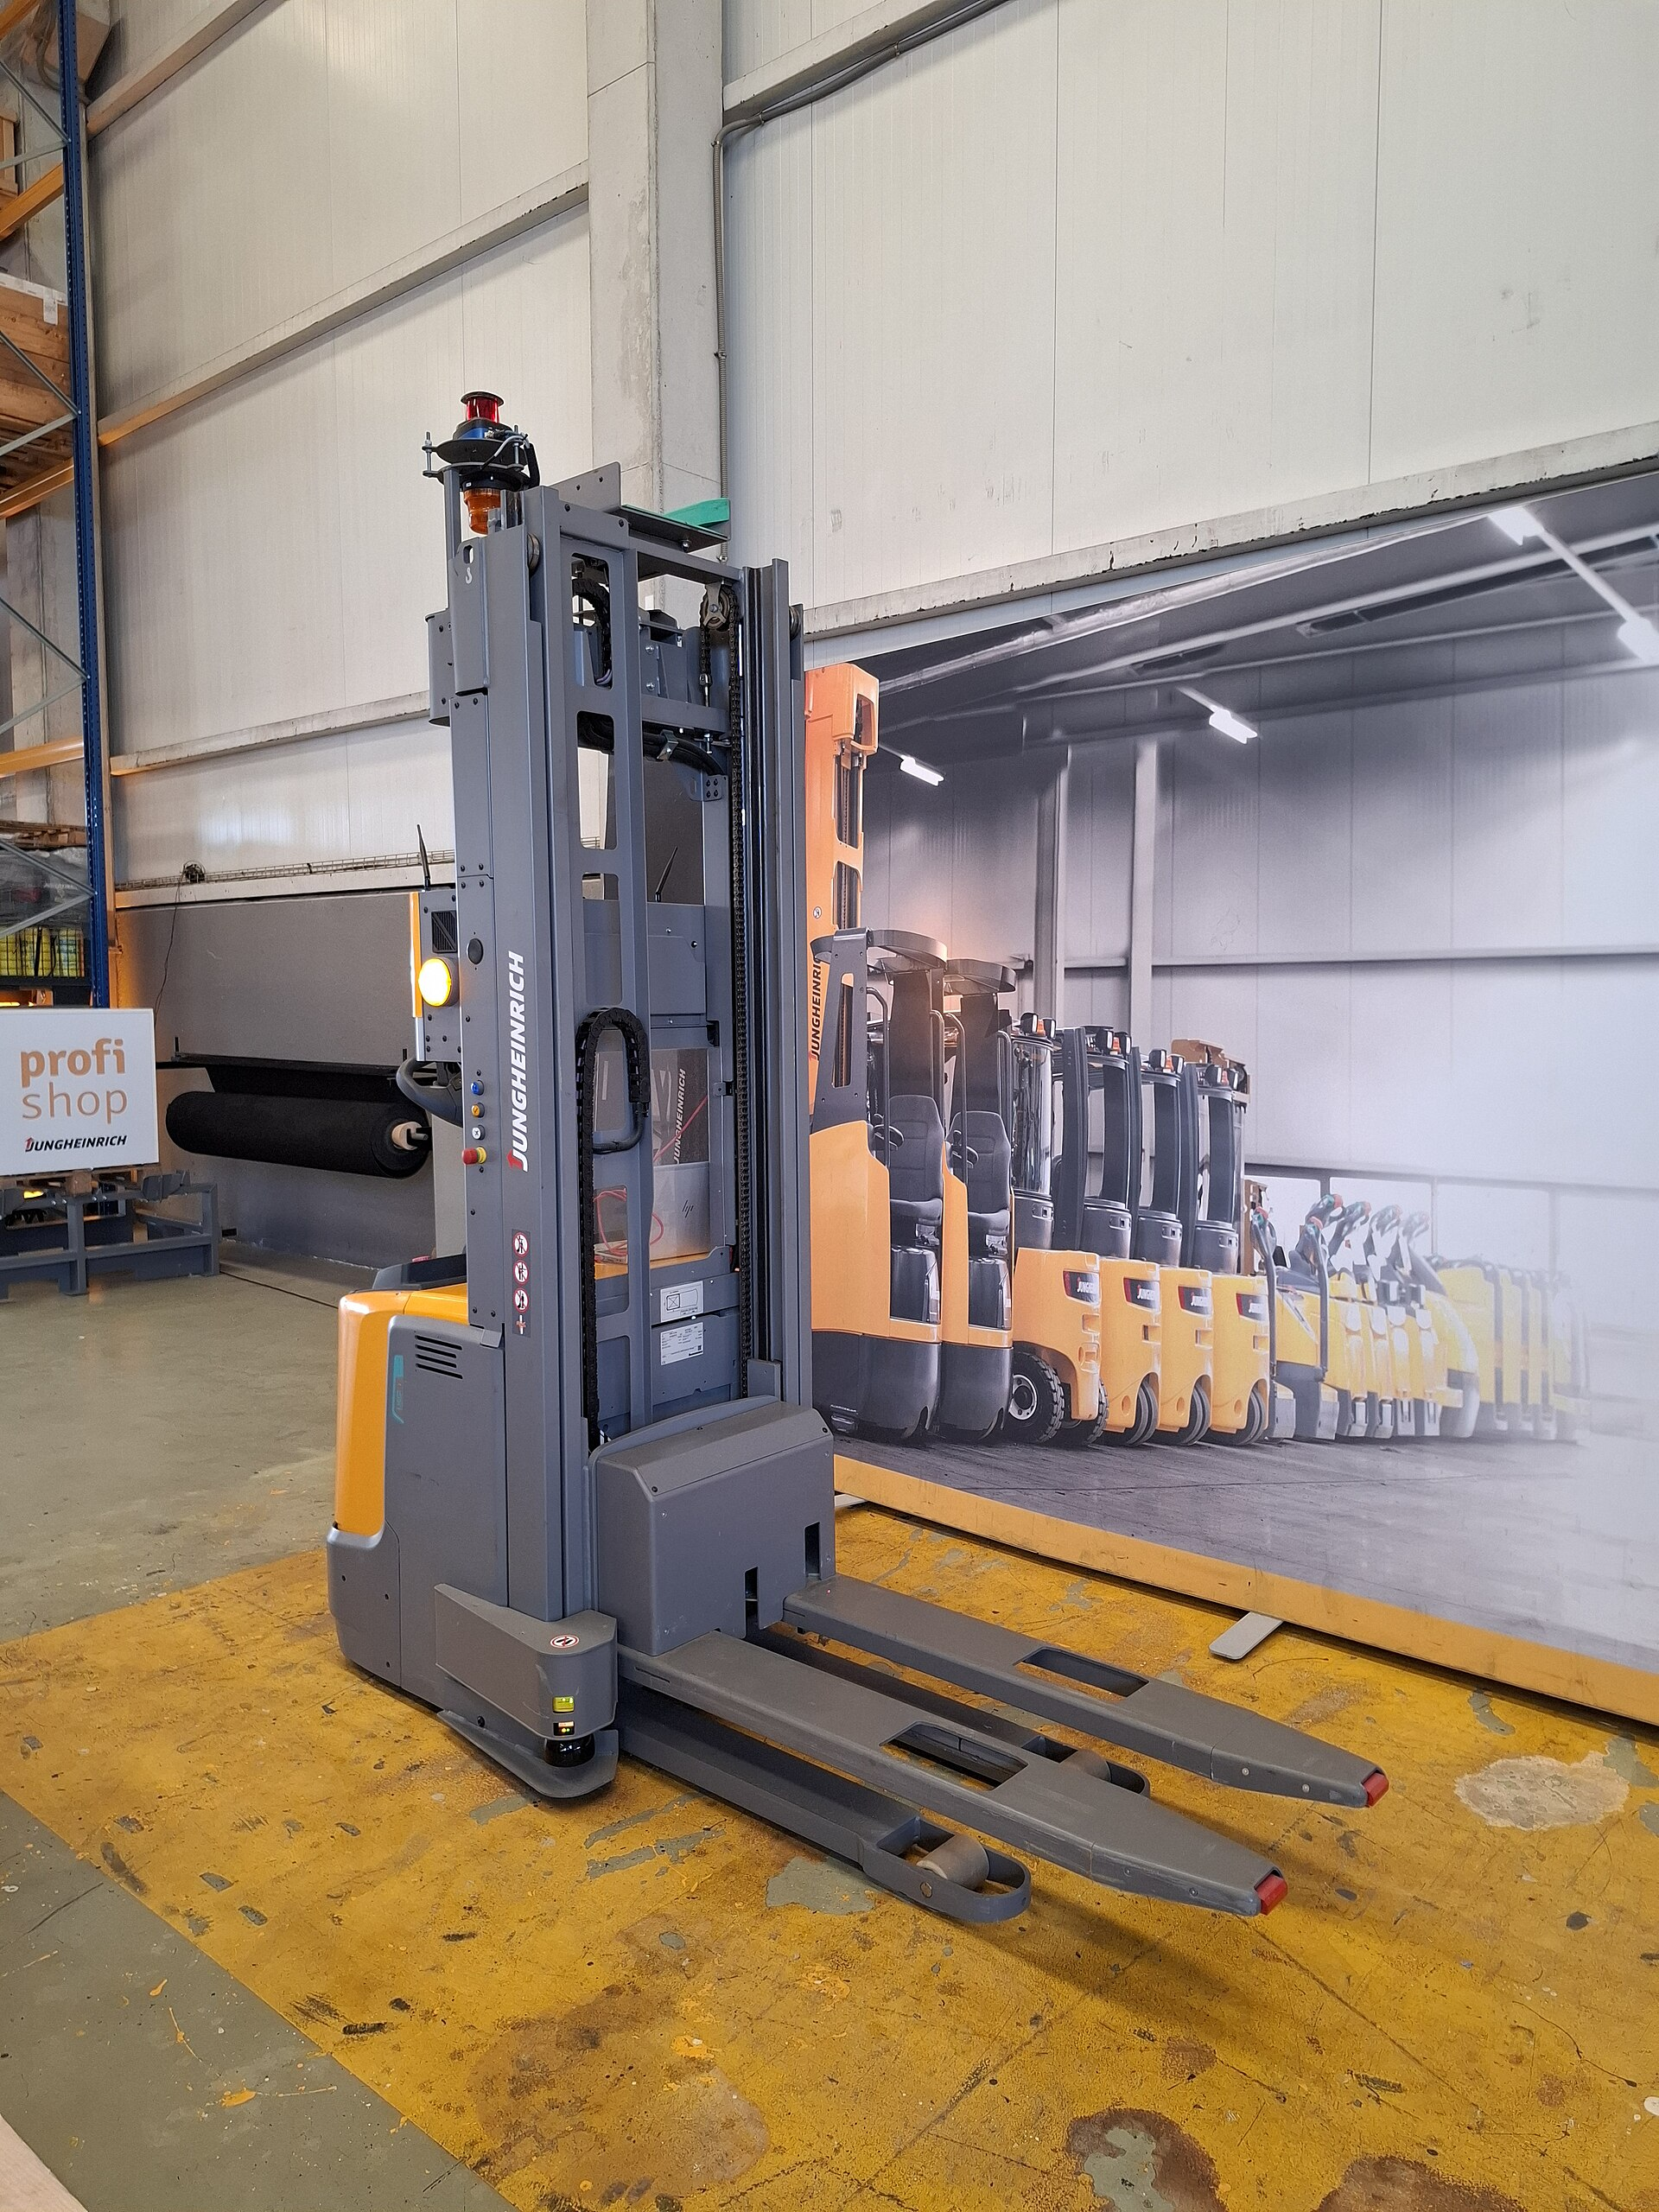
\includegraphics[height=.3\textheight]{../../figures/r22_agv.jpg}\\
\credit{\creditagv}
\column{.46\textwidth}
\begin{tikzpicture}
\begin{axis}[mkplot,width=6cm,height=5.4cm,axis equal image,xmin=-0.3,xmax=2.6,ymin=-0.3,ymax=2.6,
  xlabel={$x$ (m)},ylabel={$y$ (m)}]
\addplot[mkOrange,thick,domain=0:90,samples=40] ({2.25*sin(x)},{2.25*(1-cos(x))});
\addplot[only marks,mark=*,mkNavy,mark size=1.5pt] coordinates {(0,0) (2.25,2.25)};
\addplot[mkGray,dashed] coordinates {(0,2.25) (2.25,2.25)};
\addplot[mkGray,dashed] coordinates {(0,2.25) (0,0)};
\node[font=\tiny,anchor=south] at (axis cs:1.1,2.25) {$R=2.25$ m};
\node[font=\tiny,anchor=north west] at (axis cs:0,0) {start};
\end{axis}
\end{tikzpicture}
\end{columns}
\end{frame}

\begin{frame}[t]{Check your understanding (4.7)}
\begin{keybox}[Check your understanding]
\begin{enumerate}\small
\item A robot must apply glue along the straight edge of a car window. PTP or LIN? Why?
\item Our arm moves from A to B with a PTP move. Why does the tool not travel in a straight line?
\item An AMR has $\omega_R=\SI{5}{rad/s}$ and $\omega_L=-\SI{5}{rad/s}$ ($r=\SI{0.1}{m}$, $b=\SI{0.5}{m}$). Describe its motion.
\end{enumerate}
\end{keybox}
\end{frame}

\begin{frame}[t]{Session 4.7 summary and key terms}
\begin{columns}[T,onlytextwidth]
\column{.55\textwidth}
\begin{itemize}\small
\item Trajectory = path + timing; planner runs every few ms
\item PTP: interpolate joints, fast, curved path
\item LIN/CIRC: interpolate the TCP, IK each cycle, watch singularities
\item Gantries: trivial kinematics, large and stiff
\item Differential drive: $v$ from the wheel average, $\omega$ from the difference
\end{itemize}
\column{.41\textwidth}
\begin{defbox}[Key terms]
\small
\term{path}, \term{trajectory}, \term{PTP}, \term{LIN / CIRC}, \term{TCP}, \term{blending}, \term{jerk}, \term{gantry}, \term{differential drive}, \term{nonholonomic}
\end{defbox}
\end{columns}
\end{frame}

% =====================================================================
\section{5.1 Robotic manufacturing and flexible automation}

\begin{frame}[t]{Why automate?}
\begin{columns}[T,onlytextwidth]
\column{.5\textwidth}
\begin{itemize}\small
\item \hl{Quality}: same weld, same glue bead, every time
\item \hl{Cost}: lower cost per part at high volume, 24/7 operation
\item \hl{Safety}: the ``3 D'' jobs -- dull, dirty, dangerous
\item \hl{Speed}: shorter cycle times, faster delivery
\item Limits: high investment, needs skilled people, inflexible if badly planned
\end{itemize}
\column{.46\textwidth}
\centering
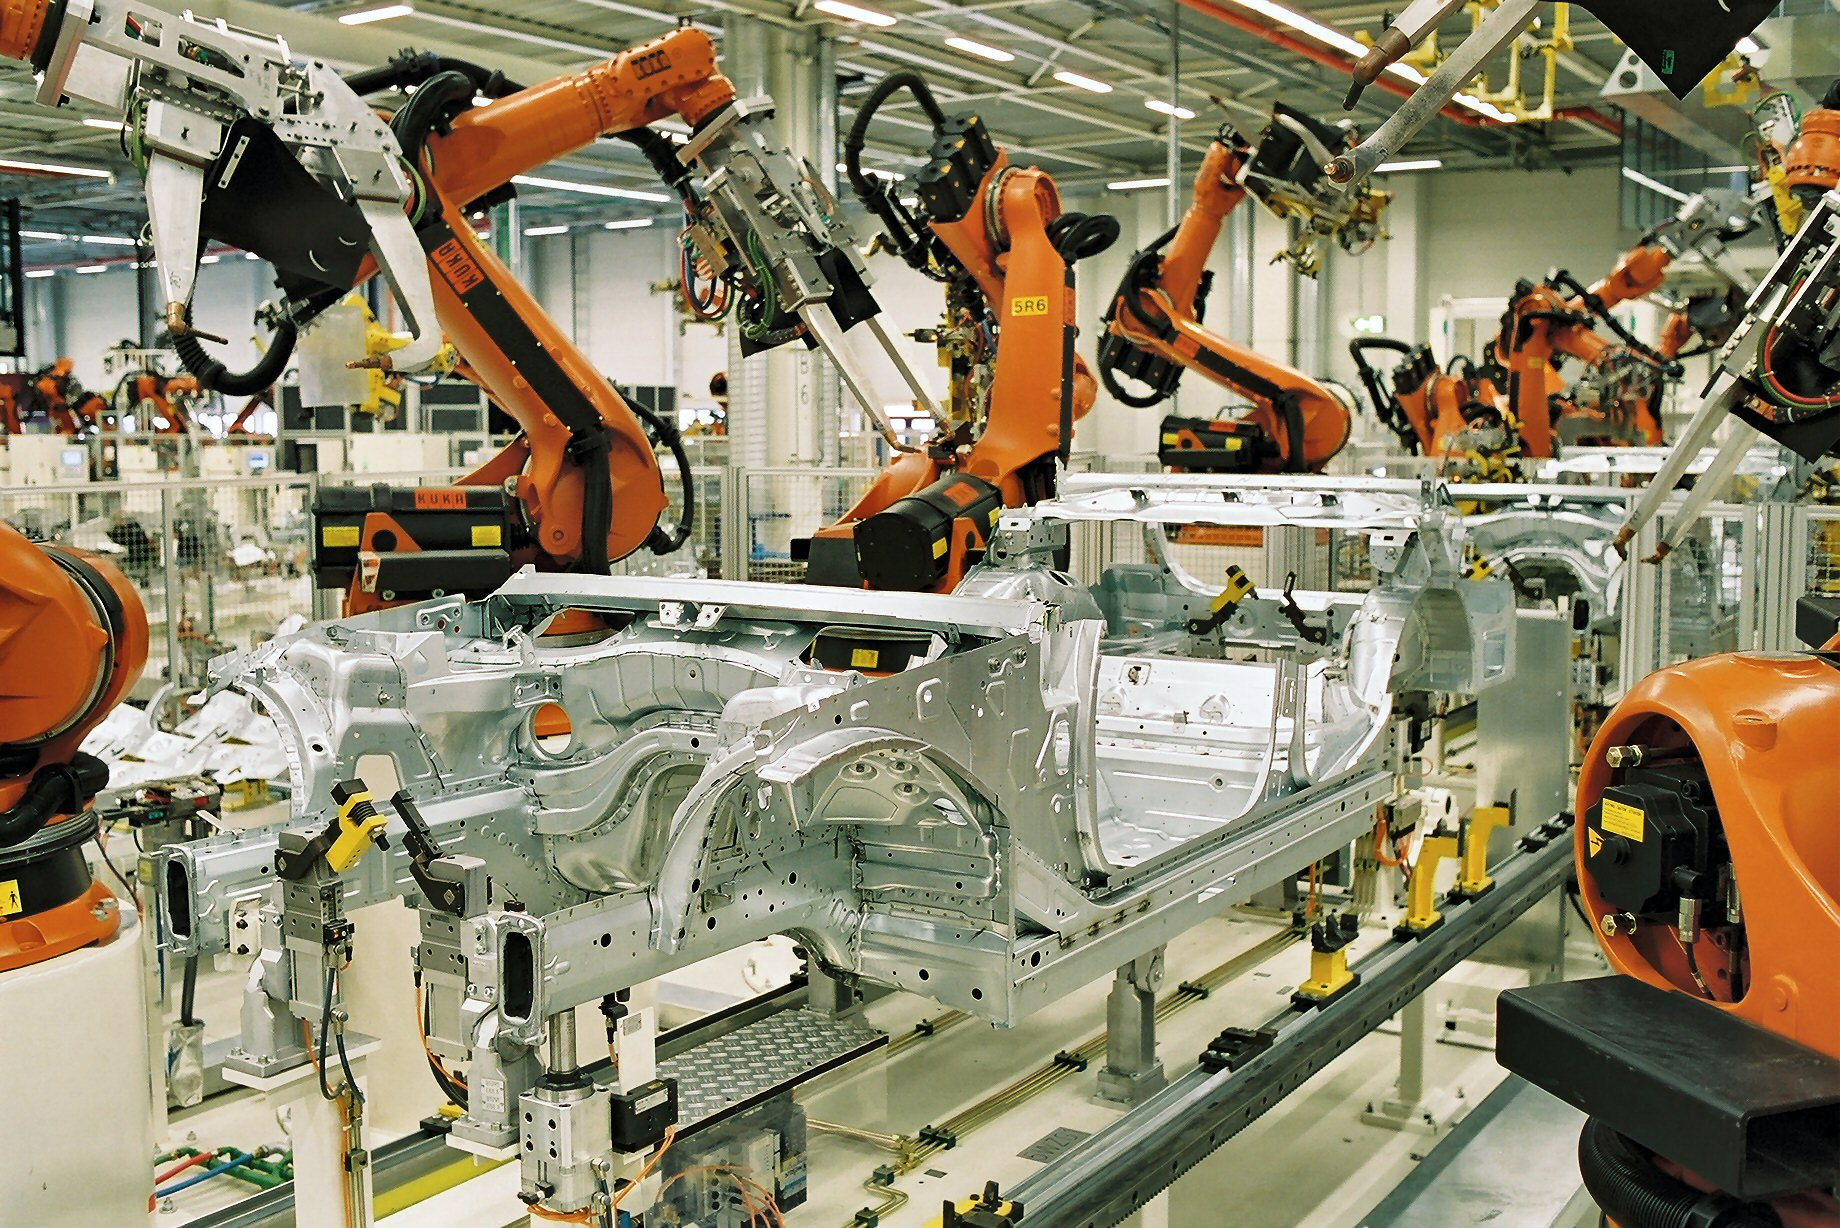
\includegraphics[width=\linewidth,height=.62\textheight,keepaspectratio]{../../figures/r22_welding.jpg}\\
\credit{\creditwelding}
\end{columns}
\end{frame}

\begin{frame}[t]{Fixed, programmable and flexible automation}
\begin{columns}[T,onlytextwidth]
\column{.48\textwidth}
\begin{itemize}\small
\item \term{Fixed (hard)}: special machine, one product, very high volume (bottle filling, transfer lines)
\item \term{Programmable}: re-programmed between \emph{batches}; changeover takes time (CNC, robots with new programs)
\item \term{Flexible}: switches between known product variants \hl{without lost time} (FMS, robot cells with tool changers)
\end{itemize}
\column{.48\textwidth}
\centering
\begin{tikzpicture}[scale=.9]
\draw[->,mkGray] (0,0) -- (5,0) node[below left,lab] {product variety};
\draw[->,mkGray] (0,0) -- (0,3.8) node[above,lab] {volume per product};
\fill[mkBlue,opacity=.25] (.1,2.6) ellipse (1.0 and .7);
\node[lab,align=center] at (.85,2.8) {fixed};
\fill[mkOrange,opacity=.3] (2.1,1.7) ellipse (1.1 and .65);
\node[lab,align=center] at (2.1,1.7) {flexible};
\fill[mkSky,opacity=.35] (3.6,.8) ellipse (1.1 and .6);
\node[lab,align=center] at (3.6,.8) {programmable};
\end{tikzpicture}
\end{columns}
\end{frame}

\begin{frame}[t]{Comparing the three types}
\centering
\small
\begin{tabularx}{.94\textwidth}{@{}l X X X@{}}
\toprule
 & \textbf{Fixed} & \textbf{Programmable} & \textbf{Flexible}\\
\midrule
Volume & very high & low to medium (batches) & medium\\
Variety & one product & many, one batch at a time & a family, mixed\\
Changeover & rebuild the machine & hours (new program, tooling) & almost none\\
Investment & high, special purpose & medium, general purpose & highest (machines + control)\\
Example & bottling line & CNC lathe, robot with new program & FMS, multi-model robot cell\\
\bottomrule
\end{tabularx}
\vspace{3mm}
\begin{notebox}
Industrial robots are \emph{programmable} machines; arranged with tool changers, vision and a cell controller they become the core of \emph{flexible} automation.
\end{notebox}
\end{frame}

\begin{frame}[t]{Worked example: when does a robot cell pay off?}
\begin{columns}[T,onlytextwidth]
\column{.47\textwidth}
\small
Cost model: total = fixed cost + cost per part $\times N$
\begin{enumerate}
\item Manual: EUR 0 + EUR 2.00 per part
\item Robot cell: EUR 150\,000 $+$ EUR 0.50 per part
\item Break-even: $2N=150\,000+0.5N$\\ $\Rightarrow N=150\,000/1.5=100\,000$ parts
\item At 400 parts/day $\rightarrow$ 250 days $\approx$ 1 year
\end{enumerate}
\begin{keybox}[Take-away]
Automation pays off with \hl{volume}. Flexibility lets one cell reach that volume with several products.
\end{keybox}
\column{.5\textwidth}
\begin{tikzpicture}
\begin{axis}[mkplot,width=6.4cm,height=5.2cm,xmin=0,xmax=200,ymin=0,ymax=400,
  xlabel={parts produced (thousands)},ylabel={total cost (k EUR)},legend pos=north west,legend cell align=left]
\addplot[mkBlue,thick,domain=0:200] {2*x};
\addlegendentry{manual}
\addplot[mkOrange,thick,domain=0:200] {150+0.5*x};
\addlegendentry{robot cell}
\addplot[only marks,mark=*,mkNavy,mark size=2pt] coordinates {(100,200)};
\node[font=\tiny,anchor=west] at (axis cs:103,190) {break-even};
\end{axis}
\end{tikzpicture}
\end{columns}
\end{frame}

\begin{frame}[t]{Flexible manufacturing systems (FMS)}
\begin{columns}[T,onlytextwidth]
\column{.56\textwidth}
\centering
\begin{tikzpicture}[scale=.82,every node/.style={font=\scriptsize}]
\node[blk,minimum width=16mm] (m1) at (0,2.4) {CNC 1};
\node[blk,minimum width=16mm] (m2) at (2.4,2.4) {CNC 2};
\node[blk,minimum width=16mm] (m3) at (4.8,2.4) {Wash /\\ inspect};
\node[blko,minimum width=16mm] (ls) at (0,-.4) {Load /\\ unload};
\node[blko,minimum width=16mm] (st) at (4.8,-.4) {Pallet\\ store};
\draw[mkMid,line width=2.5pt,rounded corners] (-1,1) -- (5.8,1);
\node[lab,fill=white] at (2.4,1) {AGV / conveyor / rail-guided vehicle};
\foreach \n in {m1,m2,m3} \draw[sig] (\n.south) -- ++(0,-.55);
\foreach \n in {ls,st} \draw[sig] (\n.north) -- ++(0,.55);
\node[blk,draw=mkNavy,fill=mkNavy,text=white,minimum width=60mm] at (2.4,-1.6) {FMS host computer: scheduling, programs, tool data};
\end{tikzpicture}
\column{.4\textwidth}
\begin{itemize}\small
\item Several CNC machines or robot cells
\item Automated material handling between them
\item Central computer routes each part
\item Runs mixed parts, often unattended at night
\end{itemize}
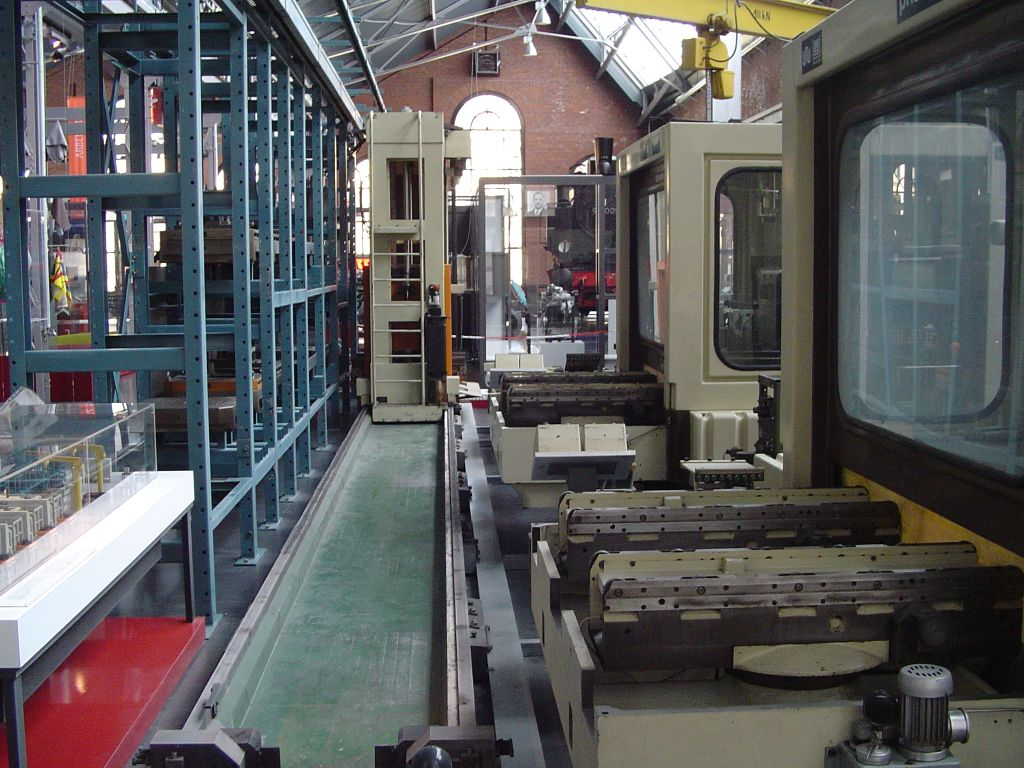
\includegraphics[width=.8\linewidth,height=.3\textheight,keepaspectratio]{../../figures/r22_fms.jpg}\\
\credit{FMS with rail-guided pallet transport. Kolossos, CC BY-SA 3.0, via Wikimedia Commons}
\end{columns}
\end{frame}

\begin{frame}[t]{Where does the robot sit? The automation pyramid}
\begin{columns}[T,onlytextwidth]
\column{.52\textwidth}
\centering
\begin{tikzpicture}[scale=.92]
\foreach \y/\w/\c/\t in {0/3.0/mkPale/{Field: sensors, motors, drives},1/2.5/mkSky!40/{Control: PLC, robot controller},2/2.0/mkSky!70/{Supervisory: SCADA, HMI},3/1.5/mkAmber!60/{MES: production orders},4/1.0/mkOrange!70/{ERP}}
 {\filldraw[fill=\c,draw=white,line width=1pt] (-\w,\y*.75) -- (\w,\y*.75) -- (\w-.5,\y*.75+.75) -- (-\w+.5,\y*.75+.75) -- cycle;
   \node[lab] at (0,\y*.75+.37) {\t};}
\draw[mkGray,<->] (3.3,0) -- (3.3,3.75);
\node[lab,rotate=90,text=mkGray] at (3.6,1.9) {ms $\leftrightarrow$ days};
\end{tikzpicture}
\column{.44\textwidth}
\begin{itemize}\small
\item Lower levels: fast (ms), small data, real-time
\item Upper levels: slow (hours, days), business data
\item Robots and PLCs at the \hl{control} level (W2D3)
\item Industrial networks connect the levels (W2D5)
\end{itemize}
\gofurther{The levels follow the ISA-95 / IEC 62264 model.}
\end{columns}
\end{frame}

\begin{frame}[t]{Industry 4.0: the connected factory}
\begin{columns}[T,onlytextwidth]
\column{.5\textwidth}
\begin{itemize}\small
\item \term{Cyber-physical system}: machine + computer + network
\item \term{Industrial IoT}: sensors on everything, data to the cloud/edge
\item \term{Digital twin}: a live simulation model of a cell (W2D3)
\item Uses: predictive maintenance, batch size one, traceability
\item Collaborative robots and AMRs make cells easy to re-arrange
\end{itemize}
\column{.46\textwidth}
\centering
\begin{tikzpicture}[xscale=1.25,yscale=.9]
\draw[mkGray,->] (0,0) -- (5.0,0);
\foreach \x/\n/\t/\y in {.4/1.0/Steam,1.7/2.0/Electricity,3.0/3.0/Electronics \& IT,4.3/4.0/Cyber-physical}{
  \fill[mkBlue] (\x,0) circle (2.5pt);
  \node[lab,above] at (\x,.15) {\textbf{\n}};
  \node[lab,below,text width=13mm,align=center] at (\x,-.15) {\t};}
\fill[mkOrange] (4.3,0) circle (3pt);
\node[lab,text=mkGray] at (2.6,1.3) {industrial revolutions};
\node[lab,text=mkGray,below] at (.4,-.9) {$\sim$1780};
\node[lab,text=mkGray,below] at (4.3,-.9) {2010s};
\end{tikzpicture}
\end{columns}
\end{frame}

\begin{frame}[t]{Measuring a production cell: cycle time and OEE}
\begin{columns}[T,onlytextwidth]
\column{.5\textwidth}
\begin{itemize}\small
\item \term{Cycle time}: time between two finished parts
\item \term{Takt time}: available time / demand -- the cycle time the customer needs
\item \term{OEE} (overall equipment effectiveness):
\end{itemize}
\begin{eqbox}
\[ \text{OEE} = \text{Availability}\times\text{Performance}\times\text{Quality} \]
\end{eqbox}
\column{.46\textwidth}
\begin{keybox}[Worked example]
\small
\begin{enumerate}
\item Shift \SI{8}{h}, demand 960 parts: takt $=28\,800/960=\SI{30}{s}$
\item Cell down 48 min: A $=432/480=0.90$
\item Runs at 95\,\% of ideal speed: P $=0.95$
\item 1\,\% scrap: Q $=0.99$
\item OEE $=0.90\cdot0.95\cdot0.99\approx0.85$
\end{enumerate}
\end{keybox}
\end{columns}
\end{frame}

\begin{frame}[t]{Check your understanding (5.1)}
\begin{keybox}[Check your understanding]
\begin{enumerate}\small
\item A bakery makes one kind of bread roll, 50\,000 per day, for years. Which type of automation fits? And a job shop making 20 different brackets in batches of 50?
\item What makes a robot cell \emph{flexible} rather than only \emph{programmable}?
\item In the break-even example, the robot cell costs EUR 0.50 per part. What happens to the break-even volume if a cheaper gripper brings it to EUR 0.25?
\end{enumerate}
\end{keybox}
\end{frame}

\begin{frame}[t]{Session 5.1 summary and key terms}
\begin{columns}[T,onlytextwidth]
\column{.55\textwidth}
\begin{itemize}\small
\item Automate for quality, cost, safety and speed
\item Fixed $\rightarrow$ programmable $\rightarrow$ flexible: more variety, less volume per product
\item Break-even: fixed cost / saving per part
\item FMS = machines + automated handling + central computer
\item Industry 4.0: connected, data-driven, re-configurable
\end{itemize}
\column{.41\textwidth}
\begin{defbox}[Key terms]
\small
\term{fixed / programmable / flexible automation}, \term{changeover}, \term{FMS}, \term{automation pyramid}, \term{Industry 4.0}, \term{digital twin}, \term{cycle time}, \term{takt time}, \term{OEE}
\end{defbox}
\end{columns}
\end{frame}

% =====================================================================
\section*{Wrap-up}

\begin{frame}[t]{Day summary}
\centering
\begin{tikzpicture}[node distance=3mm and 3mm,every node/.style={font=\scriptsize}]
\node[blk,minimum width=21mm,minimum height=12mm] (a) {\textbf{4.4 IK}\\ pose $\rightarrow$ joints\\ 2 solutions};
\node[blk,minimum width=21mm,minimum height=12mm,right=of a] (b) {\textbf{4.5 Jacobian}\\ $\bm v=J\dot{\bm\theta}$\\ $\bm\tau=J^\mathsf{T}\bm F$};
\node[blk,minimum width=21mm,minimum height=12mm,right=of b] (c) {\textbf{4.6 Dynamics}\\ $M\ddot{\bm\theta}+C\dot{\bm\theta}+\bm g$};
\node[blk,minimum width=21mm,minimum height=12mm,right=of c] (d) {\textbf{4.7 Motion}\\ PTP / LIN / CIRC\\ AMR};
\node[blko,minimum width=21mm,minimum height=12mm,right=of d] (e) {\textbf{5.1 Automation}\\ fixed / prog. / flexible};
\draw[sig] (a) -- (b); \draw[sig] (b) -- (c); \draw[sig] (c) -- (d); \draw[sig] (d) -- (e);
\end{tikzpicture}
\vspace{4mm}
\begin{columns}[T,onlytextwidth]
\column{.48\textwidth}
\begin{keybox}[Three things to remember]
\small
\begin{enumerate}
\item IK can have several answers -- or none
\item One matrix $J$ links speeds \emph{and} forces; avoid $\det J=0$
\item Gravity and payload dominate the torque of a slow arm
\end{enumerate}
\end{keybox}
\column{.48\textwidth}
\begin{defbox}[From robot to factory]
\small
The math of one arm (kinematics, dynamics, trajectories) is what makes a robot \emph{programmable}; putting robots, handling and computers together makes production \emph{flexible}.
\end{defbox}
\end{columns}
\end{frame}

\begin{frame}[t]{Preview of tomorrow (W2D3): manufacturing and automation}
\begin{columns}[T,onlytextwidth]
\column{.55\textwidth}
\begin{itemize}\small
\item \textbf{5.2} Industrial robot applications: welding, painting, palletising, machine tending, assembly, pick-and-place
\item \textbf{5.3} Work-cell design: layout, reach, cycle time, end-of-arm tooling
\item \textbf{5.4} PLCs: scan cycle, I/O, ladder logic, IEC 61131-3
\item \textbf{5.5} Robot programming: teach pendant, base/tool/user frames, offline programming, digital twin
\end{itemize}
\column{.41\textwidth}
\centering
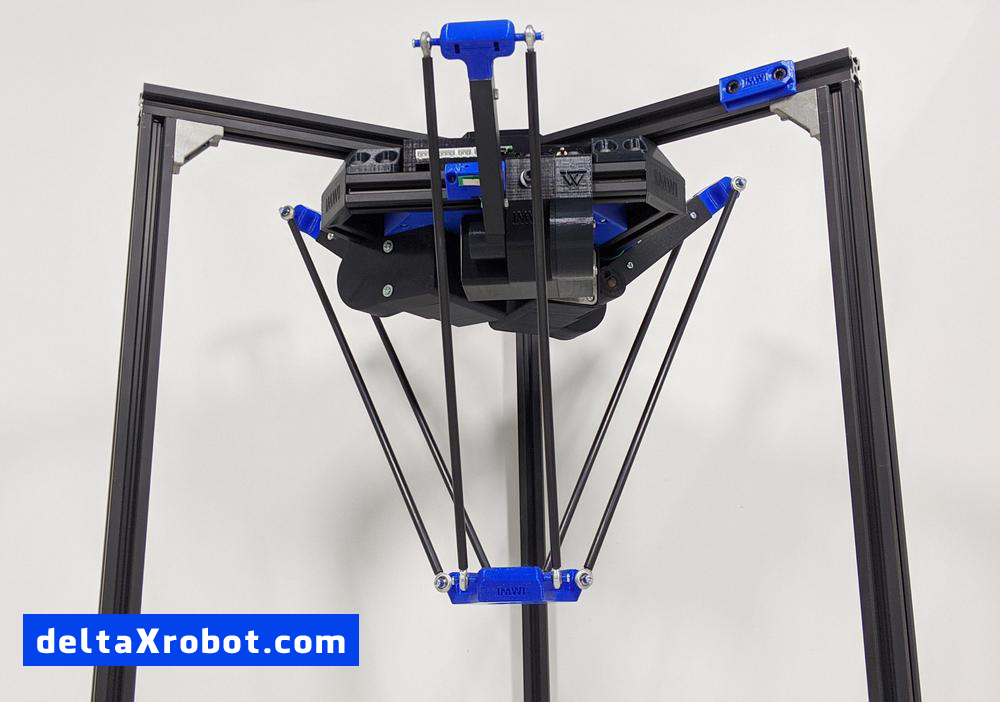
\includegraphics[width=\linewidth,height=.5\textheight,keepaspectratio]{../../figures/r22_delta.jpg}\\
\credit{Delta X robot. Trungdoanhong, CC BY-SA 4.0, via Wikimedia Commons}\\[1mm]
{\scriptsize Today's reachability check returns tomorrow as cell layout.}
\end{columns}
\end{frame}

\begin{frame}[t]{Figure credits}
\scriptsize
All photographs from Wikimedia Commons; all other drawings and plots are original (TikZ/pgfplots).
\begin{itemize}\setlength\itemsep{1pt}
\item SCARA robot (4.4): ``SCARA robot 2R.png'', Mitsubishi Electric Automation, Inc., CC BY-SA 4.0
\item KUKA industrial robot (4.5): ``KUKA industrial robotic arm performing \ldots - 02.jpg'', Oleg Yunakov, CC BY-SA 4.0
\item Mobile robot (4.7): \creditagvlong
\item Robot welding (5.1): \creditweldinglong
\item Flexible manufacturing system (5.1): ``FlexiblesFertigungssystem.jpg'', Kolossos, CC BY-SA 3.0
\item Delta robot (preview): ``Delta x robot.jpg'', Trungdoanhong, CC BY-SA 4.0
\end{itemize}
\vspace{1mm}
Full URLs: \texttt{figures/CREDITS.tsv} (lines with prefixes \texttt{r22\_} and \texttt{d4\_kuka}).
\end{frame}

\begin{frame}[t]{References}
\scriptsize
\begin{itemize}\setlength\itemsep{2pt}
\item J.\,J.~Craig, \emph{Introduction to Robotics: Mechanics and Control}, 4th ed., Pearson, 2018.
\item M.\,W.~Spong, S.~Hutchinson, M.~Vidyasagar, \emph{Robot Modeling and Control}, 2nd ed., Wiley, 2020.
\item K.\,M.~Lynch, F.\,C.~Park, \emph{Modern Robotics: Mechanics, Planning, and Control}, Cambridge University Press, 2017.
\item B.~Siciliano, L.~Sciavicco, L.~Villani, G.~Oriolo, \emph{Robotics: Modelling, Planning and Control}, Springer, 2009.
\item P.~Corke, \emph{Robotics, Vision and Control}, 3rd ed., Springer, 2023.
\item R.~Siegwart, I.\,R.~Nourbakhsh, D.~Scaramuzza, \emph{Introduction to Autonomous Mobile Robots}, 2nd ed., MIT Press, 2011.
\item M.\,P.~Groover, \emph{Automation, Production Systems, and Computer-Integrated Manufacturing}, 5th ed., Pearson, 2019.
\item ISO 9787:2013, Robots and robotic devices -- Coordinate systems and motion nomenclatures.
\item IEC 62264-1:2013, Enterprise-control system integration -- Part 1: Models and terminology.
\end{itemize}
\end{frame}

\end{document}
